\documentclass[11pt]{article}
\usepackage[a4paper,margin=22mm]{geometry}
\usepackage{fontspec}
\setmainfont{lmroman10-regular.otf}[BoldFont=lmroman10-bold.otf,ItalicFont=lmroman10-italic.otf,BoldItalicFont=lmroman10-bolditalic.otf]
\usepackage{amsmath,amssymb,amsthm,mathtools,graphicx,xcolor,hyperref,xurl,xspace}
\setlength{\emergencystretch}{4em}
\newtheorem{theo}{Theorem}[section]
\newtheorem{lemm}[theo]{Lemma}
\newtheorem{lemma}[theo]{Lemma}
\newtheorem{prop}[theo]{Proposition}
\newtheorem{coro}[theo]{Corollary}
\newtheorem{corol}[theo]{Corollary}
\newtheorem{conj}[theo]{Conjecture}
\newtheorem{Proposition}[theo]{Proposition}
\newtheorem{theoreme}[theo]{Theorem}
\theoremstyle{definition}
\newtheorem{defi}[theo]{Definition}
\newtheorem{exam}[theo]{Example}
\newtheorem{exem}[theo]{Example}
\newtheorem{rema}[theo]{Remark}
\newtheorem{nota}[theo]{Notation}
\newtheorem*{rema*}{Remark}
\newtheorem*{defi*}{Definition}
\newtheorem*{theo*}{Theorem}
\newtheorem*{lemm*}{Lemma}
\newtheorem*{prop*}{Proposition}
\newcommand{\enoncename}{}
\newtheorem{corpusenonce}[theo]{\enoncename}
\newenvironment{enonce}[1]{\renewcommand{\enoncename}{#1}\begin{corpusenonce}}{\end{corpusenonce}}
\newenvironment{enonce*}[1]{\par\medskip\noindent\textbf{#1.}\itshape}{\par\medskip}
\newenvironment{proofc}{\begin{proof}}{\end{proof}}
\newcommand{\Mc}{\mathcal{M}}
\newcommand{\pointir}{.\ ---\ }
\providecommand{\mathof}[1]{\mathrm{#1}}

\numberwithin{equation}{section}
\numberwithin{figure}{section}
\numberwithin{table}{section}
\def\endappendix{}
%~Mouliné par MaN_auto v.0.23.0 2020-06-23 16:15:44


%%\usepackage{amssymb}
%%\usepackage{cancel}
%%\usepackage{graphicx}
\usepackage{tikz}
%\usepackage{cleveref}




%\crefformat{equation}{{\rm (#2#1#3)}} %\Crefformat{equation}{{\rm (#2#1#3)}}







%%\AtBeginDocument{%\newtheorem{myname}[theo]{My beautiful theorem} }


%%\newcommand{\curl}{\operatorname{curl_{\rm 2D}}}
%%\newcommand{\grad}{\operatorname{grad}}
%%\newcommand\div{\operatorname{div}}
%%\newcommand{\sgn}{\operatorname{sgn}}
%%\newcommand{\Ker}{\operatorname{Ker}}
%%\newcommand{\Ran}{\operatorname{Ran}}


\DeclareMathOperator{\curl}{curl_{\rm{2D}}}
\DeclareMathOperator{\Div}{div}
\DeclareMathOperator{\sgn}{sgn}
\DeclareMathOperator{\Ker}{Ker}
\DeclareMathOperator{\Ran}{Ran}
\DeclareMathOperator{\grad}{grad}
\DeclareMathOperator{\Dir}{dir}
\DeclareMathOperator{\ess}{ess}
\DeclareMathOperator{\disc}{disc}
%%\DeclareMathOperator{\Min}{min}
\DeclareMathOperator{\all}{all}


%\newcommand{\Imag}{\operatorname{\mathfrak{Im}}}
%\newcommand{\Real}{\operatorname{\mathfrak{Re}}}

\newcommand{\epsl}{\varepsilon}

\newcommand{\calA}{\mathcal{A}}
\newcommand{\calC}{\mathcal{C}}
\newcommand{\calD}{\mathcal{D}}
\newcommand{\calH}{\mathcal{H}}
\newcommand{\calI}{\mathcal{I}}
\newcommand{\calJ}{\mathcal{J}}
\newcommand{\calK}{\mathcal{K}}
\newcommand{\calN}{\mathcal{N}}
\newcommand{\calR}{\mathcal{R}}
\newcommand{\calS}{\mathcal{S}}
\newcommand{\calT}{\mathcal{T}}
\newcommand{\calV}{\mathcal{V}}

\newcommand{\bbA}{\mathbb{A}}
%\newcommand{\bbB}{\mathbb{B}}
\newcommand{\bbC}{\mathbb{C}}
\newcommand{\bbN}{\mathbb{N}}
\newcommand{\bbR}{\mathbb{R}}
\newcommand{\bbS}{\mathbb{S}}
%\newcommand{\bbV}{\mathbb{V}}

\newcommand{\rmd}{{\mathrm{d}}}
\newcommand{\rmD}{{\mathrm{D}}}
\newcommand{\rme}{{\mathrm{e}}}
\newcommand{\rmm}{{\mathrm{m}}}
\newcommand{\rmi}{{\mathrm{i}}}
\newcommand{\rmp}{{\mathrm{p}}}


\newcommand{\Un}{\boldsymbol{1}}
\newcommand{\Ident}{{\mathrm{I}}}

\newcommand{\Le}{{\Lambda_{\mathrm{e}}}}
\newcommand{\Lm}{{\Lambda_{\mathrm{m}}}}

\newcounter{stepcount}
\renewcommand{\thestepcount}{\roman{stepcount}}
\newenvironment{step}{\refstepcounter{stepcount}\begin{proof}[\thestepcount]}{\let\qed\relax\end{proof}}


%%%%%%%%%%%%%%%%%%%%%%%%%%%%%%%%%%%%%%%%%%%

\graphicspath{{./figures/}}

\newcommand*{\mk}{\mkern -1mu}
\newcommand*{\Mk}{\mkern -2mu}
\newcommand*{\mK}{\mkern 1mu}
\newcommand*{\MK}{\mkern 2mu}

\hypersetup{urlcolor=purple, linkcolor=blue, citecolor=red}

\let\oldtilde\tilde
\renewcommand*{\tilde}[1]{\mathchoice{\widetilde{#1}}{\widetilde{#1}}{\oldtilde{#1}}{\oldtilde{#1}}}
%\let\oldhat\hat
%\renewcommand*{\hat}[1]{\mathchoice{\widehat{#1}}{\widehat{#1}}{\oldhat{#1}}{\oldhat{#1}}}
\let\oldexists\exists
\renewcommand*{\exists}{\mathrel{\oldexists}}
\let\oldforall\forall
\renewcommand*{\forall}{\mathrel{\oldforall}}


\newcommand*{\romanenumi}{\renewcommand*{\theenumi}{\roman{enumi}}}
\newcommand*{\Romanenumi}{\renewcommand*{\theenumi}{\Roman{enumi}}}
\newcommand*{\alphenumi}{\renewcommand*{\theenumi}{\alph{enumi}}}
\newcommand*{\Alphenumi}{\renewcommand*{\theenumi}{\Alph{enumi}}}

%%%%%%%%%%%%%%%%%%%%%%%%%%%%%%%%%%%%%%%%%%%%%

\begin{document}
\section*{\raggedright 2637: The half magnetic Drude parameter lies in the essential spectrum of the augmented operator for polygonal two-material cavities with nonintersecting interfaces}
\noindent\textbf{Author:} Christophe Hazard; Sandrine Paolantoni\par\noindent\textbf{Source:} Spectral analysis of polygonal cavities containing a negative-index material. Annales Henri Lebesgue 3 (2020), publisher version, DOI 10.5802/ahl.58. \url{https://ahl.centre-mersenne.org/item/AHL_2020__3__1161_0/}
\par\noindent\textbf{License:} CC BY 4.0, \url{https://creativecommons.org/licenses/by/4.0/}. The original publisher PDF has the explicit license notice. See the saved source/license records.
\par\noindent\textbf{Editorial material note (not author text):} The selected problem is Proposition 3.6: the planar-interface Weyl sequence for the half magnetic Drude parameter in the essential spectrum of the augmented selfadjoint operator, with the exact polygonal-cavity, nonintersecting-interface, positivity and coupled-domain hypotheses. The complete author body retains the local augmented-operator setup, surface-wave superposition, transmission-domain, defect, nonvanishing-gradient and weak-convergence estimates. Other corner-spectrum and nonlinear-pencil assertions are unselected. Original TikZ diagrams remain editable; one unrelated wave illustration is a figure-only publisher clip with native editable caption, never a source-page wrapper. All proof text and formulas below are editable author TeX. Mathematical wording, language and proof order are retained. Only the article class, title matter and bibliography presentation are adapted for independent compilation; no proof has been generated or repaired.
\par\noindent\textbf{Editorial difficulty:} H1: The source constructs Fourier superpositions of exponentially confined interface waves, verifies the nonstandard coupled transmission operator domain, and proves concentration with a nonvanishing gradient norm and weak convergence to create an essential-spectrum Weyl sequence. This spectral resonance mechanism for a dispersive augmented PDE operator exceeds ordinary qualifying problems.
\par\noindent\textbf{Editorial retrieval and attribution:} Retrieved 2026-10-01. DOI 10.5802/ahl.58. Source attribution notice: ../licenses/2637-source-license.txt; complete legal text: ../licenses/CC-BY-4.0.txt. Original source excerpts and the existing source-material check are retained in ../sources/2637/.
\medskip\hrule\medskip
\noindent\textbf{Author statement, complete proof and local supporting text follow in source order.}
\section{Introduction}\label{s-intro}
An electromagnetic \emph{negative-index material} (NIM), often also called left-handed material, is a material whose microscopic structure leads to an unusual macroscopic behavior: in some frequency range(s), both macroscopic electric permittivity and magnetic permeability (or at least their real parts) become \emph{negative}. Such materials were first introduced theoretically in the late sixties by Veselago~\cite{Ves-68} who exhibited the concept of negative refraction. The potentialities of NIMs for practical applications were investigated about 30 years later, mainly after the famous paper by Pendry~\cite{Pen-00} who opened the quest for spectacular devices such as the perfect flat lens or the invisibility cloak. Since then, these extraordinary materials have generated a great effervescence among the communities of physicists and mathematicians. Surprisingly very little has been achieved in the spectral analysis of systems involving a NIM. The present paper intends to bring a contribution in this framework. Its purpose is to show on a simple example that the presence of an interface between a NIM and a usual material is responsible for an \emph{essential spectrum}.

One inherent difficulty of the spectral analysis of NIMs follows from an intrinsic physical property of such materials: \emph{frequency dispersion}. Indeed, an electromagnetic NIM is necessarily a dispersive material in the sense that in the frequency domain, its permittivity and permeability (thus also the wave velocity) depend on the frequency. As a consequence, contrary to the case of a usual dielectric medium, the time-harmonic Maxwell's equations depend non-linearly on the frequency. Hence, when looking for the spectrum of an electromagnetic device involving a NIM, one has to solve a non-linear eigenvalue problem. This issue is very rarely mentioned in the mathematical literature. Indeed, most existing works concern the behavior of NIMs in the frequency domain, that is, propagation of time-harmonic waves at a given frequency. Our study relies on these works, which enlighten the fundamental role played by the \emph{contrasts}, that is, the respective ratios of permittivity and permeability across the interface. The first study in this context is due to Costabel and Stephan~\cite{Cos-Ste-85} in the mid-eighties. They considered a scalar transmission problem (which involves only one contrast) and showed by an integral equation technique that in the case of a smooth interface, the transmission problem is well-posed if and only if the contrast is different from the critical value $-1.$ The detailed study of this critical value of the contrast is achieved in~\cite{Ola-95} and more recently in~\cite{Cac-Pan-Pos}, both for smooth interfaces. The case of a two-dimensional non-smooth interface was tackled about fifteen years after the pioneering work of Costabel and Stephan: it was understood in~\cite{Bon-Dau-Ram-99} that in the presence of a corner, this critical value becomes a critical interval (which contains $-1)$ depending on the angle of the corner. About another fifteen years later, the elegant T-coercivity technique gave a new light on these critical sets for two- and three-dimensional scalar transmission problems~\cite{Bon-Che-Cia-12,Ngu-16}, as well as Maxwell's equations~\cite{Bon-Che-Cia-14a,Bon-Che-Cia-14b}. An alternative point of view, based on the so-called Neumann--Poincaré operator, has received recently a resurgence of interest~\cite{Amm-etal-13,And-Kan-16,Amm-Mil-Rui-Zha-17,Bon-Zha-17,Per-Put-17}: it provides another way to investigate these critical sets. From a physical point of view, the critical sets of the contrast are related to remarkable physical phenomena. On the one hand, the critical value $-1$ associated to a smooth interface ensures the existence of surface waves (localized near the interface) called \emph{surface plasmons}~\cite{Gra-May-12,Gri-14}. On the other hand, the critical interval associated with a corner on the interface gives rise to a possible concentration of energy near the vertex, which has been interpreted as a ``black hole'' effect at the corner~\cite{Bon-etal-16}.

There are very few papers in the literature which deal directly with the non-linear eigenvalue problem resulting from \emph{frequency dispersion}. Let us cite for instance~\cite{Coc-Maz-Mou-12} where some generic well-posedness results are established thanks to Fredholm's analytical theory, with various applications to metamaterials. In cases where the dependence on the spectral parameter is rational, it is possible to get rid of the spectral non-linearity by introducing suitable auxiliary fields. The initial non-linear eigenvalue problem can then be re-written as a linear one which involves both original and auxiliary fields. This \emph{augmented formulation} technique actually comes within a general approach for rational operator valued functions which can be related with block operator matrices. It has a long history which seems to start at the end of the 70's with the concept of \emph{transfer function}~\cite{Bar-Goh-Kaa-79} and was then widely developed under the name \emph{Schur complement} borrowed from the theory of matrices~\cite{Nag-89,Tre-08}. Similar ideas also apply for the numerical solution of rational eigenvalue problems~\cite{Gut-Tis-17,Su-Bai-11}. From a theoretical point of view, this approach was used for instance in~\cite{Ada-Lan-95} to study completeness properties of a family of eigenvectors of a rational operator valued function. More recently, it is developed in~\cite{Eng-Lan-Tre-17} to establish min-max characterizations of eigenvalues of some kinds of rational operator functions, with applications to photonics which are closed to the problem addressed in the present paper. The augmented formulation approach is used in~\cite{Cas-Haz-Jol} to achieve a complete spectral analysis of Maxwell's equations in the case of a plane interface between a NIM and vacuum. It is also developed in~\cite{Bru-Gra-Dem-16} to perform the numerical calculation of modes for cavities or photonic crystals containing a dissipative NIM. Let us finally mention that in the context of Maxwell's equations, the idea of introducing auxiliary fields was investigated by Tip~\cite{Tip-98} in dissipative and dispersive linear media. Compared to the Schur complement technique, the originality of the augmented formulation proposed by Tip concerns dissipative problems for which a suitable choice of auxiliary variables leads to a \emph{selfadjoint} operator. The same idea applies actually in a very wide frame of systems~\cite{Fig-Sch-07} which observe two fundamental assumptions: causality (causes precede effects) and passivity (nothing comes from nothing).



The aim of the present paper is to explore the spectrum of the \emph{linear augmented formulation} constructed from the initial \emph{non-linear} eigenvalue problem, considering an elementary situation. Firstly, instead of the three-dimensional Maxwell's equations, we deal with a two-dimensional scalar equation (which can be derived from Maxwell's equations in a medium which is invariant in one space direction). Secondly, we choose the simplest existing model of NIM, namely the non dissipative Drude model, for which negativity occurs at low frequencies. Finally, we consider the case of a bounded cavity consisting of two polygonal parts: one part filled with a Drude material and the complementary part filled with vacuum. We will see that contrary to a cavity filled with a usual dielectric (for which the spectrum is always purely discrete: it is made of a sequence of positive eigenvalues which tends to $+\infty),$ the presence of the Drude material gives rise to various components of an \emph{essential spectrum} corresponding to various unusual \emph{resonance} phenomena:

\begin{enumerate}\romanenumi
\item \label{list1.1}A low frequency \emph{bulk resonance}: the zero frequency is an accumulation point of positive eigenvalues whose associated eigenvectors are confined in the Drude material.

\item \label{list1.2}A \emph{surface resonance}: for the particular frequency which corresponds to the critical value $-1$ of the contrast, localized highly oscillating vibrations are possible near any ``regular point'' of the interface between the Drude material and the vacuum (by ``regular point'', we mean a point which is not a vertex of a corner).

\item \label{list1.3}A \emph{corner resonance}: for any frequency in the frequency intervals which correspond to the critical intervals of the contrast associated to each corner, localized highly oscillating vibrations are possible near the vertex, which is related to the ``black hole'' phenomenon.
\end{enumerate}

A crucial issue will remain open at the end of the paper: what is the relation between the essential spectrum of the \emph{linear augmented formulation} studied here and that of the initial \emph{non-linear problem}? Can we deduce from our results that the latter has the same components of essential spectrum? In some situations, the answer to such a question follows from general results (which is one of the main objectives of spectral theory of block operator matrices, see~\cite{Tre-08}). Unfortunately, none of these general results applies to our situation and we are unable to give here a satisfying answer to this delicate question.

The paper is organized as follows. In Section~\ref{s-formulation}, we present our scalar problem as well as its augmented formulation and give the main results of the paper. Section~\ref{s-investigation} is devoted to the proof of these results, which mainly consists in investigating the above mentioned resonance phenomena using the notion of \emph{Weyl sequences}. We conclude with some perspectives. Finally Appendix~\ref{s-appendix} presents a short discussion about the tricky question of the relation between the respective essential spectra of both linear and non-linear problems.

Throughout the paper, we use the following notations for usual functional spaces. For an open set $\Omega \subset \bbR^d$ $(d \ge 1),$ we denote by $\calD(\Omega)$ the space of infinitely differentiable functions with compact support contained in $\Omega,$ by $L^2(\Omega)$ the space of square integrable functions in $\Omega,$ by $H^s(\Omega),$ for $s \in \bbR,$ the usual Sobolev space of order $s$ and by $H^1_0(\Omega)$ the closure of $\calD(\Omega)$ in $H^1(\Omega).$ Moreover, in order to avoid the appearance of non meaningful constants in inequalities, we employ the symbols $\lesssim$ and $\gtrsim$ which mean that the inequality is satisfied up to a positive factor which does not depend on the parameters involved in the inequality (for instance, $|f(x)| \lesssim 1$ means that $f$ is bounded).


\section{Formulation of the problem and main results}\label{s-formulation}

\subsection{Original non-linear problem}\label{s-nonlinear}
Our aim is to study the spectral properties of a two-dimensional bounded cavity partially filled with a NIM. We consider a polygonal cavity $\calC$ (bounded open set of $\bbR^2)$ divided into two open polygonal domains $\calN$ and $\calV$ (such that $\overline{\calN} \cup \overline{\calV} = \overline{\calC}$ and $\calN \cap \calV = \emptyset,$ see Figure~\ref{f.cavity}). As these notations suggest, $\calN$ and $\calV$ are filled respectively with a NIM and vacuum. We denote by $\Sigma$ the interface between $\calN$ and $\calV$ (that is, $\Sigma := \partial\calN \cap \partial\calV),$ which clearly consists of one or several polygonal curve(s). In the case of several curves, we assume that they do not intersect (in particular checkerboard-like cavities are excluded).
\begin{figure}[!b]
\begin{center}
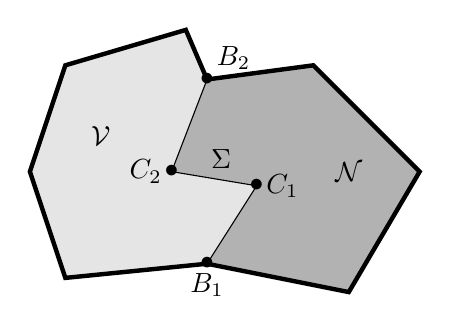
\begin{tikzpicture}[scale=0.9]
\fill [gray!60] (2.,0.2) -- (4.,-0.2) -- (5.,1.5) -- (3.5,3.) -- (2.,2.8) -- (1.5,1.5) -- (2.7,1.3) -- cycle;
\fill [gray!20] (0.,0.) -- (2.,0.2) -- (2.7,1.3) -- (1.5,1.5) -- (2.,2.8) -- (1.7,3.5) -- (0.,3.) -- (-0.5,1.5) -- cycle;
\draw [ultra thick] (0.,0.) -- (2.,0.2) -- (4.,-0.2) -- (5.,1.5) -- (3.5,3.) -- (2.,2.8) -- (1.7,3.5) -- (0.,3.) -- (-0.5,1.5) -- cycle;
\draw (2.,0.2) -- (2.7,1.3) -- (1.5,1.5) -- (2.,2.8);
\draw (2.,0.2) node {$\bullet$} node[below] {$B_1$};
\draw (2.7,1.3) node {$\bullet$} node[right] {$C_1$};
\draw (1.5,1.5) node {$\bullet$} node[left] {$C_2$};
\draw (2.,2.8) node {$\bullet$} node[above right] {$B_2$};
\draw (2.2,1.4) node [above] {$\Sigma$};
\draw (0.5,2) node {$\calV$};
\draw (4,1.5) node {$\calN$};
\end{tikzpicture}
\hspace{5mm}
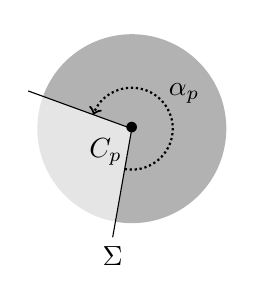
\begin{tikzpicture}[scale=0.4]
\fill[fill=gray!60] (0,0) -- (-100:3) arc (-100:160:3);
\fill[fill=gray!20] (0,0) -- (160:3) arc (160:260:3);
\draw[->,thick,densely dotted] (-100:1.3) arc (-100:160:1.3);
\draw (-100:3.5) -- (0,0) -- (160:3.5);
\draw (30:1) node[above right] {$\alpha_p$};
\draw (0,0) node{$\bullet$} node[below left] {$C_p$};
\draw (-100:3.5) node[below] {$\Sigma$};
\end{tikzpicture}
\hspace{5mm}
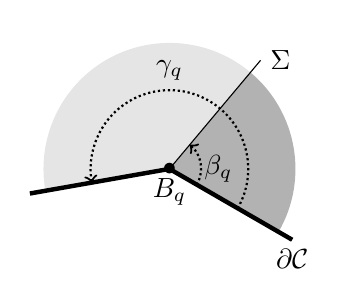
\begin{tikzpicture}[scale=0.4]
\fill[fill=gray!60] (0,0) -- (-30:4) arc (-30:50:4);
\fill[fill=gray!20] (0,0) -- (50:4) arc (50:190:4);
\draw[->,thick,densely dotted] (-30:1.) arc (-30:50:1.);
\draw[->,thick,densely dotted] (-30:2.5) arc (-30:190:2.5);
\draw [ultra thick] (-30:4.5) -- (0,0) -- (190:4.5);
\draw (0,0) -- (50:4.5);
\draw (0:0.8) node[right] {$\beta_q$};
\draw (90:2.5) node[above] {$\gamma_q$};
\draw (0,0) node{$\bullet$} node[below] {$B_q$};
\draw (50:4.5) node[right] {$\Sigma$};
\draw (-30:4.5) node[below] {$\partial\calC$};
\end{tikzpicture}
\end{center}
\caption{Left: The polygonal cavity $\calC$ divided into $\calN$ (NIM: dark gray) and $\calV$ (vacuum: light gray). Middle: an inner vertex $C_p$ of the interface $\Sigma$ between $\calN$ and $\calV.$ Right: a boundary vertex $B_q$ of $\Sigma.$}\label{f.cavity}
\end{figure}

We consider in this paper the simplest model of NIM, known as the non-dissipative Drude model, for which the electric permittivity and the magnetic permeability are respectively defined in the frequency domain by
\begin{equation}\label{e.Drude-model}
\epsl^\calN_\lambda := \epsl_0\, \left(1 - \frac{\Le}{\lambda} \right)
\quad\text{and}\quad
\mu^\calN_\lambda := \mu_0\, \left(1 - \frac{\Lm}{\lambda} \right),
\end{equation}
where $\lambda := \omega^2$ denotes the square of the (circular) frequency, $\epsl_0$ and $\mu_0$ are the permittivity and the permeability of the vacuum and the coefficients $\Le$ and $\Lm$ are positive constants which characterize the Drude material. Such a material is a negative material at low frequencies (since $\epsl^\calN_\lambda < 0$ if $0 < \lambda < \Le,$ respectively $\mu^\calN_\lambda < 0$ if $0 < \lambda < \Lm)$ and behaves like the vacuum at high frequencies (since $\epsl^\calN_\lambda \to \epsl_0$ and $\mu^\calN_\lambda \to \mu_0$ when $\lambda \to +\infty).$ Note that the ratio $\mu^\calN_\lambda/\mu_0$ (respectively, $\epsl^\calN_\lambda/\epsl_0)$ is equal to the critical value $-1$ if $\lambda = \Lm/2$ (respectively, $\lambda = \Le/2$).

In $\calV,$ the permittivity and permeability are those of the vacuum, which leads us to introduce two piecewise constant functions defined in the cavity $\calC$ by
\begin{equation}\label{e.def-eps-mu}
\epsl_\lambda(x) := \epsl_0\, \left(1 - \Un_\calN(x)\,\frac{\Le}{\lambda} \right)
\quad\text{and}\quad
\mu_\lambda(x) := \mu_0\, \left(1 - \Un_\calN(x)\,\frac{\Lm}{\lambda} \right)
\end{equation}
for $x \in \calC,$ where $\Un_\calN$ denotes the indicator function of $\calN.$ The starting point of our study is the following eigenvalue problem, which describes the \emph{resonances} of the cavity:
\begin{align}
& \text{Find } \lambda \in \bbC \text{ and a nonzero } \varphi \in H^1_0(\calC) \text{ such that} \nonumber \\
& \Div \left(\frac{1}{\mu_\lambda}\, \grad\varphi \right) + \lambda\,\epsl_\lambda\,\varphi = 0
\quad\text{in }\calC. \label{e.NLin}
\end{align}
The latter equation has to be understood in the distributional sense. In other words, the above problem is a condensed form of the following system:
\begin{subequations}
\begin{align}
 \Delta\varphi + \lambda\,\epsl_\lambda^\calN \mu_\lambda^\calN\, \varphi &= 0
\quad\text{in }\calN, \label{e.Helm.N}
\\ \Delta\varphi + \lambda\,\epsl_0 \mu_0\,\varphi &= 0
\quad\text{in }\calV, \label{e.Helm.V}
\\
[\varphi]_\Sigma &= 0 \text{ and } \left[\frac{1}{\mu_\lambda}\,\frac{\partial\varphi}{\partial n} \right]_\Sigma = 0, \label{e.transm.NV}
\\ 
\varphi &= 0 \quad\text{on }\partial\calC, \label{e.Diri}
\end{align}
\end{subequations}
where $[f]_\Sigma$ denotes the jump of a function $f$ across $\Sigma,$ that is, the difference of the traces of $f$ obtained from both sides. In the transmission conditions~\eqref{e.transm.NV},\linebreak$n$ denotes a unit normal to $\Sigma.$ These conditions couple the Helmholtz equations~\eqref{e.Helm.N} and~\eqref{e.Helm.V} on both sides of $\Sigma.$ The Dirichlet boundary condition~\eqref{e.Diri} is contained in the choice of the Sobolev space $H^1_0(\calC)$ for $\varphi.$

The above eigenvalue problem is clearly \emph{non-linear} with respect to $\lambda,$ unless $\calN$ is empty (i.e., $\calC$ only contains vacuum). In this latter case, \eqref{e.NLin} is linear since it reduces to \eqref{e.Helm.V}-\eqref{e.Diri}, which means that $\lambda\,\epsl_0\mu_0$ is an eigenvalue of the Dirichlet Laplacian, that is, the selfadjoint operator $-\Delta^{\!\Dir}$ defined by
\[
-\Delta^{\!\Dir} \varphi := -\Delta \varphi,
\quad\forall \varphi \in \rmD(-\Delta^{\!\Dir}) := \Big\{ \varphi \in H^1_0(\calC); \
\Delta\varphi \in L^2(\calC) \Big\}.
\]
It is well known that the spectrum $\sigma(-\Delta^{\!\Dir})$ of this operator is purely discrete: it is composed of a sequence of positive eigenvalues of finite multiplicity which tends to $+\infty.$

On the other hand, if $\calV = \emptyset$ (i.e., if $\calC$ only contains the Drude material), \eqref{e.NLin} reduces to~\eqref{e.Helm.N}-\eqref{e.Diri}, which means that $\lambda\,\epsl_\lambda^\calN \mu_\lambda^\calN$ is an eigenvalue the operator $-\Delta^{\!\Dir}$ defined above. Hence the set of eigenvalues of our non-linear problem is simply the inverse image of $\sigma(-\Delta^{\!\Dir})$ under the function $f$ defined by
\begin{equation}
f(\lambda) := \lambda\,\epsl_\lambda^\calN \mu_\lambda^\calN = \lambda\,\epsl_0\mu_0 \left(1 - \frac{\Le}{\lambda} \right)
\left(1 - \frac{\Lm}{\lambda} \right),\label{e.def-f}
\end{equation}
which is represented in Figure~\ref{f.inv-image-f}. As $f(\lambda)$ tends to $+\infty$ when $\lambda$ goes to 0 or $+\infty$, the eigenvalues accumulate at $+\infty$ as well as 0.
\begin{figure}
\begin{center}
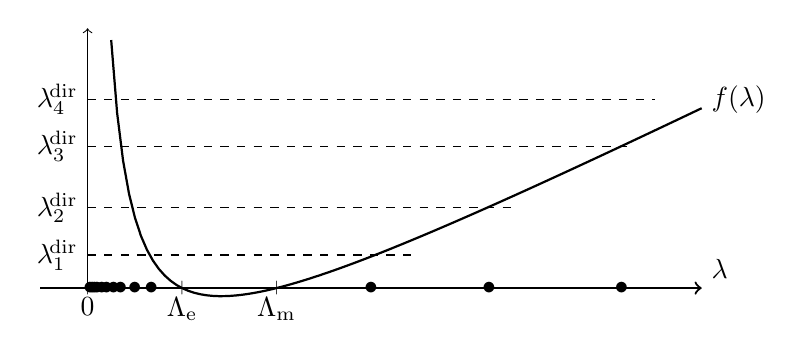
\begin{tikzpicture}[scale=0.6]
\draw [->=latex,thick] (-1,0) -> (13,0);
\draw [->=latex,thin] (0,0) -> (0,5.5);
\draw [thick,samples=100,domain=0.5:13] plot (\x, \x/2 - 3 + 4/ \x);
\draw [dashed] (0,0.7) -- (7,0.7);
\draw [dashed] (0,1.7) -- (9,1.7);
\draw [dashed] (0,3) -- (11.5,3);
\draw [dashed] (0,4) -- (12,4);
\draw (0,0) node{$\scriptscriptstyle |$};
\draw (2,0) node{$\scriptscriptstyle |$};
\draw (4,0) node{$\scriptscriptstyle |$};
\draw (0,0) node[below]{$0$};
\draw (2,0) node[below]{$\Le$};
\draw (4,0) node[below]{$\Lm$};
\draw (13,0) node[above right]{$\lambda$};
\draw (13,4) node[right]{$f(\lambda)$};
\draw (0,0.7) node[left]{$\lambda_1^{\!\Dir}$};
\draw (0,1.7) node[left]{$\lambda_2^{\!\Dir}$};
\draw (0,3) node[left]{$\lambda_3^{\!\Dir}$};
\draw (0,4) node[left]{$\lambda_4^{\!\Dir}$};
\draw (0.05,0) node {$\bullet$};
\draw (0.1,0) node {$\bullet$};
\draw (0.15,0) node {$\bullet$};
\draw (0.2,0) node {$\bullet$};
\draw (0.3,0) node {$\bullet$};
\draw (0.4,0) node {$\bullet$};
\draw (0.55,0) node {$\bullet$};
\draw (0.7,0) node {$\bullet$};
\draw (1,0) node {$\bullet$};
\draw (1.35,0) node {$\bullet$};
\draw (6,0) node {$\bullet$};
\draw (8.5,0) node {$\bullet$};
\draw (11.3,0) node {$\bullet$};
\end{tikzpicture}
\end{center}
\caption{The dots on the $\lambda$-axis represent the inverse image of $\sigma(-\Delta^{\!\Dir})= \{ \lambda_n^{\!\Dir};\, n \geq 1 \}$ under the function $f$ defined in~\eqref{e.def-f} (in the case $\Lambda_{\mathrm{e}} < \Lambda_{\mathrm{m}}$).}\label{f.inv-image-f}
\end{figure}

Of course, when both vacuum and Drude material are present in the cavity, such simple arguments can no longer be used. As mentioned in the introduction, general techniques of block operator matrices allow us to transform the non-linear eigenvalue problem~\eqref{e.NLin} into a \emph{linear} one which involves a \emph{selfadjoint} operator, thanks to the introduction of an additional unknown. This is the object of the following subsection~\ref{s-linear}.

\subsection{Linearization of the problem}\label{s-linear}

Let us first introduce some notations. We denote by $\calR: L^2(\calC) \to L^2(\calN)$ the operator of restriction from $\calC$ to $\calN$ and by $\calR^*: L^2(\calN) \to L^2(\calC)$ the operator of extension by 0 from $\calN$ to $\calC,$ that is, for all $(\varphi,\psi) \in L^2(\calC) \times L^2(\calN),$
\[
\calR \varphi := \varphi|_\calN
\quad\text{and}\quad
\calR^* \psi(x) :=
\begin{cases}
\psi(x) & \text{if }x \in \calN, \\
0 & \text{if }x \in \calV.
\end{cases}
\]
These operators are clearly adjoint to each other since
\[
\int_\calN \calR \varphi(x) \, \overline{\psi(x)} \,\rmd x = \int_\calC \varphi(x) \, \overline{\calR^* \psi(x)} \,\rmd x.
\]
Note that $\calR \calR^*$ is the identity in $L^2(\calN),$ whereas $\calR^* \calR$ is the operator of multiplication by $\Un_\calN$ in $L^2(\calC).$ We shall keep the same notations $\calR$ and $\calR^*$ if $\varphi$ and $\psi$ are replaced by vector-valued functions in $L^2(\calC)^2 \times L^2(\calN)^2.$

The construction of a linear eigenvalue problem equivalent to~\eqref{e.NLin} is quite simple. We assume in the sequel that $\lambda \neq \Lm,$ so that $\mu_\lambda^{-1}$ remains bounded. Note that for $\lambda = 0,$ problem~\eqref{e.NLin} still makes sense provided we replace $(\mu^\calN_\lambda)^{-1}$ and $\lambda\,\epsl^\calN_\lambda$ by their limiting values, respectively, $0$ and $-\epsl_0\Le$. Using the definition~\eqref{e.def-eps-mu} of $\epsl_\lambda$ and $\mu_\lambda,$ which shows in particular that
\[
\frac{1}{\mu_\lambda} = \frac{1}{\mu_0}\,\left(1 + \Un_\calN\,\frac{\Lm}{\lambda-\Lm}\right),
\]
we can rewrite~\eqref{e.NLin} in the form
\[
\frac{1}{\epsl_0 \mu_0}\,\Div \left\{ \left(1 + \Un_\calN\,\frac{\Lm}{\lambda-\Lm}\right) \grad\varphi \right\} + \left(\lambda - \Un_\calN\,\Le \right)\,\varphi = 0.
\]
Hence, setting
\begin{equation}
u := \frac{\Lm}{\lambda-\Lm} \calR \grad\varphi,\label{e.def-u}
\end{equation}
equation~\eqref{e.NLin} is equivalent to
\begin{subequations}
\begin{align}
\frac{-1}{\epsl_0 \mu_0}\,\Div \left\{ \grad\varphi + \calR^* u \right\} &+ \Un_\calN\,\Le\,\varphi= \lambda\,\varphi \quad\text{in }\calC, \label{e.Lin-one}
\\
\Lm\,\calR\grad\varphi &+ \Lm\,u\quad\;= \lambda\,u \quad\,\text{in }\calN, \label{e.Lin-two}
\end{align}
\end{subequations}
where the latter equation is nothing but the definition~\eqref{e.def-u} of $u.$ In this system of equations, $\lambda$ only appears in the right-hand side: it is a \emph{linear} eigenvalue problem for the pair $(\varphi,u).$ To sum up, if $\lambda \neq \Lm,$ a function $\varphi \in H^1_0(\calC)$ is a solution to~\eqref{e.NLin} if and only if $(\varphi,u) \in H^1_0(\calC) \times L^2(\calN)^2$ satisfies
\begin{equation}
\bbA
\begin{pmatrix} \varphi \\ u
\end{pmatrix}
= \lambda \
\begin{pmatrix} \varphi \\ u
\end{pmatrix}\label{e.Lin}
\end{equation}
where
\begin{equation}\label{e.defA}
\bbA
\begin{pmatrix} \varphi \\ u
\end{pmatrix}
:=
\begin{pmatrix}
\displaystyle \frac{-1}{\epsl_0 \mu_0}\,\Div \left\{\grad\varphi + \calR^* u \right\} + \Un_\calN\,\Le\,\varphi \\[8pt]
\Lm\,\calR \grad\varphi + \Lm\,u
\end{pmatrix}.
\end{equation}
It remains to make precise the proper functional framework in which $\bbA$ is selfadjoint. Consider the Hilbert space
\[
\calH := L^2(\calC) \times L^2(\calN)^2
\]
equipped with the inner product
\begin{equation}\label{e.def-inner-prod}
\Big((\varphi,u), (\varphi',u') \Big)_\calH :=
\epsl_0 \mu_0 \, \int_\calC \varphi(x) \, \overline{\varphi'(x)} \,\rmd x + \frac{1}{\Lm} \, \int_\calN u(x) \cdot \overline{u'(x)} \,\rmd x.
\end{equation}

\begin{prop}
The operator $\bbA$ defined by~\eqref{e.defA} with domain
\begin{equation}\label{e.def-Dom-A}
\rmD(\bbA) := \Big\{ (\varphi,u) \in H^1_0(\calC) \times L^2(\calN)^2; \
\Div(\grad \varphi + \calR^* u) \in L^2(\calC) \Big\}
\end{equation}
is selfadjoint and non-negative in $\calH$.\label{p.A-selfadjoint}
\end{prop}

\begin{proof}
Consider the following sesquilinear form $a$ defined for all pairs $\Phi := (\varphi,u)$ and $\Phi' := (\varphi',u')$ in $\rmD(a) := H^1_0(\calC) \times L^2(\calN)^2$ equipped with the usual norm, denoted by $\| \cdot \|_{\rmD(a)}$:
\[
a(\Phi,\Phi') :=
\int_\calC (\grad\varphi + \calR^*u) \cdot \overline{(\grad\varphi' + \calR^* u')}\,\rmd x + \Le \varepsilon_0 \mu_0 \int_\calN \varphi \, \overline{\varphi'} \, \rmd x.
\]
Thanks to Green's formula, we deduce from the definition~\eqref{e.defA} of $\bbA$ that
\begin{equation}\label{e.formesymA}
(\bbA \Phi, \Phi')_\calH = a(\Phi,\Phi')
\quad \forall \Phi \in \rmD(\bbA), \quad \forall \Phi' \in \rmD(a).
\end{equation}
It is clear that $a$ is continuous, non-negative and symmetric in $\rmD(a),$ which is continuously embedded in $\calH.$ Hence, if there exist $\lambda \in \bbR$ and $m>0$ such that
\begin{equation}\label{e.coercivite}
a(\Phi,\Phi) + \lambda \| \Phi \|_\calH^2 \geq m \| \Phi \|_{\rmD(a)}^2
\quad \forall \Phi \in \rmD(a),
\end{equation}
it is well-known~\cite[Theorem~2.1, p.~322]{Kato-84} that~\eqref{e.formesymA} defines a unique non-negative selfadjoint operator $\bbA$ with domain
\[
\rmD(\bbA) := \big\{ \Phi \in \rmD(a);\ \exists \Psi \in \calH,\ \forall \Phi' \in \rmD(a), \ a(\Phi,\Phi')=(\Psi,\Phi')_\calH \big\}.
\]
It is easy to see that this definition coincide with~\eqref{e.def-Dom-A}. In order to check inequality~\eqref{e.coercivite}, note that for any $\lambda > 0,$ we have
\begin{multline*}
\left\| \grad \varphi + \calR^* u\right\|_{L^2(\calC)}^2 =
\left\| \sqrt{\frac{\Lm}{\lambda}} \grad \varphi + \sqrt{\frac{\lambda}{\Lm}} \calR^* u\right\|_{L^2(\calC)}^2 \\
+ \left(1 - \frac{\Lm}{\lambda} \right) \| \grad \varphi\|_{L^2(\calC)}^2 + \left(1 - \frac{\lambda}{\Lm} \right) \| u \|_{L^2(\calN)}^2.
\end{multline*}
As a consequence,
\[
a(\Phi,\Phi) + \lambda \| \Phi \|_\calH^2
\geq \left(1 - \frac{\Lm}{\lambda} \right) \| \grad \varphi\|_{L^2(\calC)}^2 + \lambda \varepsilon_0 \mu_0\, \| \varphi \|_{L^2(\calC)}^2 + \| u \|_{L^2(\calN)}^2.
\]
So, if $\lambda>\Lm$, inequality~\eqref{e.coercivite} holds with $m = \min (1- \Lm/\lambda, \lambda \varepsilon_0 \mu_0, 1).$
\end{proof}



Summing up, the above linearization process amounts to identifying the \emph{point spectrum} $\sigma_{\rmp}(\bbA)$ of $\bbA$ with that of a rational family of operators associated to the original non-linear problem~\eqref{e.NLin}. It seems natural to consider here the family\linebreak$\bbC\setminus\{\Lm\} \ni \lambda \mapsto \bbS_\lambda$ of unbounded operators defined in $L^2(\calC)$ by
\begin{align}
\rmD(\bbS_\lambda) & := \big\{ \varphi \in H^1_0(\calC); \ \Div(\mu_\lambda^{-1}\grad \varphi) \in L^2(\calC) \big\} \quad \text{and} \label{e.def-DomS}
\\
\bbS_\lambda \varphi & := -\Div \left(\mu_\lambda^{-1}\, \grad\varphi \right) - \lambda\,\epsl_\lambda\,\varphi
\quad\forall \varphi \in \rmD(\bbS_\lambda). \label{e.def-S}
\end{align}

Thus if we define
\begin{equation}
\sigma_{\rmp}(\bbS_\lambda) := \big\{ \lambda \in \bbC\setminus\{\Lm\};\ \Ker(\bbS_\lambda)\neq\{0\} \big\},\label{e.spectre-ponct-S}
\end{equation}
we have proved that $\sigma_{\rmp}(\bbS_\lambda) = \sigma_{\rmp}(\bbA)\setminus\{\Lm\}.$

Proposition~\ref{p.A-selfadjoint} tells us that the spectrum $\sigma(\bbA)$ of $\bbA$ is real and non-negative. Contrary to the case of a cavity filled by ordinary materials, this spectrum is not only \emph{discrete}. The rest of the paper is precisely to describe and analyze the content of the \emph{essential spectrum} $\sigma_{\ess}(\bbA)$ of $\bbA.$ The latter should reasonably be expected to coincide with that of $\bbS_\lambda.$ Unfortunately, we are not able to prove rigorously such a plausible assertion. Some explanations about this awkward question are given in the~Appendix~\ref{s-appendix}.

\subsection{Main results}\label{s-main-results}
Recall (see, e.g., \cite{Edm-Eva-87}) that the \emph{discrete spectrum} $\sigma_{\disc}(\bbA)$ is the set of isolated eigenvalues of finite multiplicity. The \emph{essential spectrum} is its complement in the spectrum, that is, $\sigma_{\ess}(\bbA) := \sigma(\bbA) \setminus \sigma_{\disc}(\bbA),$ which contains either accumulation points of the spectrum or isolated eigenvalues of infinite multiplicity. Our study of $\sigma_{\ess}(\bbA)$ is based on a convenient characterization of the essential spectrum: a real number $\lambda$ belongs to $\sigma_{\ess}(\bbA)$ if and only if there exists a sequence $(\Phi_n)_{n \in \bbN} \subset \rmD(\bbA)$ such that
\begin{equation*}
\| \Phi_n \|_\calH = 1, \quad
\lim_{n\to\infty} \| \bbA \Phi_n - \lambda \Phi_n \|_\calH = 0
\quad\text{and}\quad
\lim_{n\to\infty} (\Phi_n,\Psi)_\calH = 0, \ \forall\Psi\in\calH,
\end{equation*}
which is called a \emph{Weyl sequence} for $\lambda$ (or a \emph{singular sequence}). The two first conditions actually characterize any point of $\sigma(\bbA),$ whereas the last one (weak convergence to~$0$) is specific to $\sigma_{\ess}(\bbA).$

We summarize below the main results of the paper about the various components of $\sigma_{\ess}(\bbA).$

First, the value $\lambda = \Lm$ is an eigenvalue of infinite multiplicity of $\bbA$ (see Proposition~\ref{p.partic-values}). The non-linear eigenvalue problem~\eqref{e.NLin} does not make sense for this particular value, since $\mu_\lambda^{-1}$ becomes infinite in $\calN.$ We will see that this eigenvalue of $\bbA$ is actually an \emph{artifact} of the augmented formulation (see Remark~\ref{r-artifact}).

The other components of $\sigma_{\ess}(\bbA)$ correspond to various unusual \emph{resonance} phenomena. A \emph{bulk resonance} in the Drude material corresponds to the value $\lambda = 0,$ which is an accumulation point of the discrete spectrum. A \emph{surface resonance} at the interface $\Sigma$ between $\calN$ and $\calV$ corresponds to the value $\lambda = \Lm/2$. Finally, a \emph{corner resonance} at every vertex of the interface $\Sigma$ gives rise to a continuous set in the essential spectrum. To make this set precise, we have to distinguish between the \emph{inner vertices} $\{ C_p \in \Sigma;\, p=1,\ldots,P \}$ located inside $\calC$ and the \emph{boundary vertices} $\{ B_q \in \Sigma;\, q=1,\ldots,Q \}$ located on the boundary $\partial\calC$ (see Figure~\ref{f.cavity}). On the one hand, for an inner vertex $C_p,$ the corner resonance is observed in two intervals which are symmetric with respect to $\Lm/2$:
\begin{align}
\calJ_p &:= \left\{ \lambda \in \bbR;\ 0 < \left|\lambda-\frac{\Lm}{2}\right| < \frac{\Lm}{2}\left|1-\frac{\alpha_p}{\pi}\right| \right\} \label{e.def-J_p}
\\
&\;= \left]
\frac{\Lm}{2}\left(1-\left|1-\frac{\alpha_p}{\pi}\right|\right),
\frac{\Lm}{2}
\right[
\cup
\left]
\frac{\Lm}{2},
\frac{\Lm}{2}\left(1+\left|1-\frac{\alpha_p}{\pi}\right|\right)
\right[, \nonumber
\end{align}
where $\alpha_p \in (0,2\pi)\setminus \{ \pi \}$ denotes the angle of the Drude sector as shown in Figure~\ref{f.cavity}. We see that if $\alpha_p$ is close to 0 or $2\pi$ (which means that the corner is sharp either in $\calN$ or in $\calV$), this set fills almost $]0,\Lm[\setminus \{\Lm/2\}$, whereas if $\alpha_p$ is close to $\pi,$ this set concentrates near $\Lm/2$ (it becomes empty if $\alpha_p = \pi,$ i.e., no corner). On the other hand, for a boundary vertex $B_q,$ the corner resonance is observed in only one interval defined by
\begin{equation}\label{e.def-I_q}
\calI_q := \left]
\frac{\Lm}{2}\, \min\left(1,\frac{2\beta_q}{\gamma_q} \right),
\frac{\Lm}{2}\, \max\left(1,\frac{2\beta_q}{\gamma_q} \right)
\right[,
\end{equation}
where the angles $\beta_q, \gamma_q \in (0,2\pi)$ are defined in Figure~\ref{f.cavity}. As above, if $\beta_q /\gamma_q$ is close to 0 (respectively, to 1), this set fills almost $]0,\Lm/2[$ (respectively $]\Lm/2,\Lm[)$, whereas if $\beta_q/\gamma_q$ is close to $1/2$, this set concentrates near $\Lm/2$ and becomes empty if $\beta_q = \gamma_q/2$.

The main result of this paper is the following Theorem~\ref{theo2.2} whose proof is the subject of the next section~(in particular Section~\ref{s.proof-thm}).
\begin{theo}\label{theo2.2}
Suppose that $\calN \neq \emptyset$ and $\calV \neq \emptyset.$ Then the essential spectrum $\sigma_{\ess}(\bbA) \subset \sigma(\bbA) \subset [0,+\infty)$ of $\bbA$ is given by
\[
\sigma_{\ess}(\bbA) = \left\{0,\Lm/2,\Lm \right\} \ \cup \bigcup_{p=1,\,P} \overline{\calJ_p}
\ \cup \bigcup_{q=1,\,Q} \overline{\calI_q}.
\]
Moreover the eigenvalues of the discrete spectrum $\sigma_{\disc}(\bbA)$ accumulate at $0$ and $+\infty.$\label{th.main}
\end{theo}

\begin{figure}
\begin{center}
\begin{tabular}{ccc}
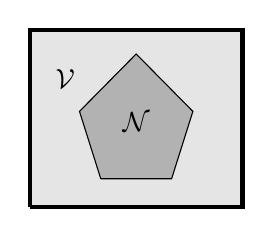
\begin{tikzpicture}[scale=0.9]
\fill [fill=gray!20,draw=black,ultra thick] (-1,-0.4)--(2,-0.4)--(2,2.1)--(-1,2.1)--(-1,-0.4);
\fill [fill=gray!60,draw=black] (0,0)--(1,0)--(1.3,0.95)--(0.5,1.76)--(-0.3,0.95)--(0,0);
\node[text=black] (n1) at (-0.5,1.4) {$\calV$};
\node[text=black] (n1) at (0.5,0.8) {$\calN$};
\end{tikzpicture} &
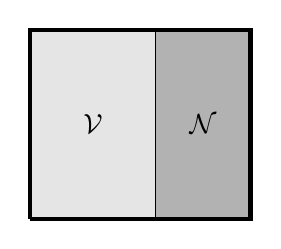
\begin{tikzpicture}[scale=0.4]
\fill [fill=gray!60,draw=black] (4,0)--(7,0)--(7,6)--(4,6)--(4,0);
\fill [fill=gray!20,draw=black] (0,0)--(4,0)--(4,6)--(0,6)--(0,0);
\draw [ultra thick] (0,0)--(7,0)--(7,6)--(0,6)--(0,0);
\node[text=black] (n1) at (2,3) {$\calV$};
\node[text=black] (n1) at (5.5,3) {$\calN$};
\end{tikzpicture} &
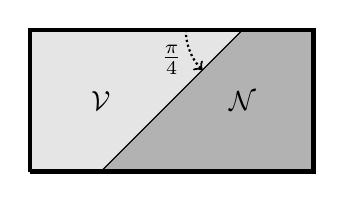
\begin{tikzpicture}[scale=1.8]
\fill [fill=gray!60,draw=black] (1,0)--(2.5,0)--(2.5,1)--(2,1)--(1,0);
\fill [fill=gray!20,draw=black] (0.5,0)--(1,0)--(2,1)--(0.5,1)--(0.5,0);
\draw [ultra thick] (0.5,0)--(2.5,0)--(2.5,1)--(0.5,1)--(0.5,0);
\node[text=black] (n1) at (1,0.5) {$\calV$};
\node[text=black] (n1) at (2,0.5) {$\calN$};
\node[text=black] (n1) at (1.5,0.79) {$\frac{\pi}{4}$};
\begin{scope}[shift={(2,1)}]
\draw[->,thick,densely dotted] (180:0.4) arc (180:225:0.4);
\end{scope}
\end{tikzpicture}
\vspace{2mm}
\\
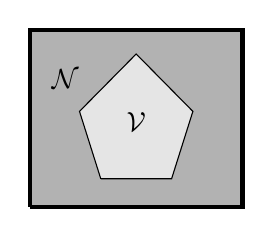
\begin{tikzpicture}[scale=0.9]
\fill [fill=gray!60,draw=black,ultra thick] (-1,-0.4)--(2,-0.4)--(2,2.1)--(-1,2.1)--(-1,-0.4);
\fill [fill=gray!20,draw=black] (0,0)--(1,0)--(1.3,0.95)--(0.5,1.76)--(-0.3,0.95)--(0,0);
\node[text=black] (n1) at (-0.5,1.4) {$\calN$};
\node[text=black] (n1) at (0.5,0.8) {$\calV$};
\end{tikzpicture} &
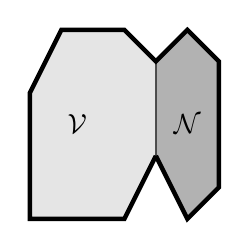
\begin{tikzpicture}[scale=0.4]
\fill [fill=gray!60,draw=black] (4,2)--(5,0)--(6,1)--(6,5)--(5,6)--(4,5)--(4,2);
\fill [fill=gray!20,draw=black] (0,0)--(3,0)--(4,2)--(4,5)--(3,6)--(1,6)--(0,4)--(0,0);
\draw [ultra thick] (4,2)--(5,0)--(6,1)--(6,5)--(5,6)--(4,5)--(3,6)--(1,6)--(0,4)--(0,0)--(3,0)--(4,2);
\node[text=black] (n1) at (1.5,3) {$\calV$};
\node[text=black] (n1) at (5,3) {$\calN$};
\end{tikzpicture} &
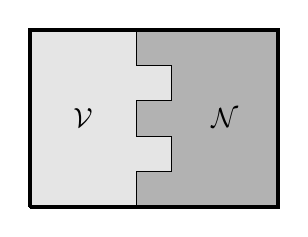
\begin{tikzpicture}[scale=0.45]
\fill [fill=gray!60,draw=black] (3,0)--(7,0)--(7,5)--(3,5)--(3,4)--(4,4)--(4,3)--(3,3)--(3,2)--(4,2)--(4,1)--(3,1)--(3,0);
\fill [fill=gray!20,draw=black] (3,0)--(0,0)--(0,5)--(3,5)--(3,4)--(4,4)--(4,3)--(3,3)--(3,2)--(4,2)--(4,1)--(3,1)--(3,0);
\draw [ultra thick] (0,0)--(7,0)--(7,5)--(0,5)--(0,0);
\node[text=black] (n1) at (1.5,2.5) {$\calV$};
\node[text=black] (n1) at (5.5,2.5) {$\calN$};
\end{tikzpicture}
\\
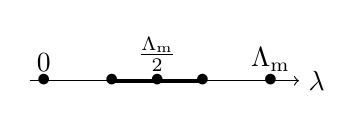
\begin{tikzpicture}[scale=0.36]
\draw [->=latex] (-0.5,0) -> (9,0);
\draw [ultra thick] (2.4,0) -- (5.6,0);
\draw (0,0) node {$\bullet$} node[above] {$0$};
\draw (8,0) node {$\bullet$} node[above] {$\Lm$};
\draw (4,0) node {$\bullet$} node[above] {$\frac{\Lm}{2}$};
\draw (2.4,0) node {$\bullet$};
\draw (5.6,0) node {$\bullet$};
\draw (9,0) node[right] {$\lambda$};
\end{tikzpicture} &
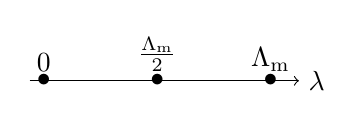
\begin{tikzpicture}[scale=0.36]
\draw [->=latex] (-0.5,0) -> (9,0);
\draw (0,0) node {$\bullet$} node[above] {$0$};
\draw (8,0) node {$\bullet$} node[above] {$\Lm$};
\draw (4,0) node {$\bullet$} node[above] {$\frac{\Lm}{2}$};
\draw (9,0) node[right] {$\lambda$};
\end{tikzpicture} &
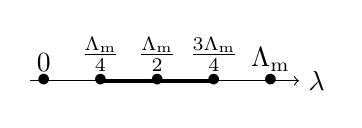
\begin{tikzpicture}[scale=0.36]
\draw [->=latex] (-0.5,0) -> (9,0);
\draw [ultra thick] (2,0) -- (6,0);
\draw (0,0) node {$\bullet$} node[above] {$0$};
\draw (8,0) node {$\bullet$} node[above] {$\Lm$};
\draw (4,0) node {$\bullet$} node[above] {$\frac{\Lm}{2}$};
\draw (2,0) node {$\bullet$} node[above] {$\frac{\Lm}{4}$};
\draw (6,0) node {$\bullet$} node[above] {$\frac{3\Lm}{4}$};
\draw (9,0) node[right] {$\lambda$};
\end{tikzpicture}
\end{tabular}
\end{center}
\caption{Examples of cavities leading to an essential spectrum which is symmetric with respect to $\Lm/2$. Each column shows two different cavities leading to the same essential spectrum represented by dots and a thick line on the $\lambda$-axis.}\label{ex1}
\end{figure}

\begin{figure}
\begin{center}
\begin{tabular}{cc}
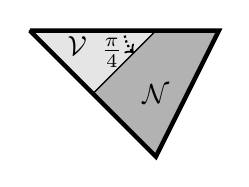
\begin{tikzpicture}[scale=0.4]
\fill [fill=gray!60,draw=black] (2,2)--(4,0)--(6,4)--(4,4)--(2,2);
\fill [fill=gray!20,draw=black] (2,2)--(4,4)--(0,4)--(2,2);
\draw [ultra thick] (0,4)--(4,0)--(6,4)--(0,4);
\node[text=black] (n1) at (1.5,3.5) {$\calV$};
\node[text=black] (n1) at (4,2) {$\calN$};
\node[text=black] (n1) at (2.6,3.3) {$\frac{\pi}{4}$};
\begin{scope}[shift={(4,4)}]
\draw[->,thick,densely dotted] (180:1) arc (180:225:1);
\end{scope}
\end{tikzpicture} &
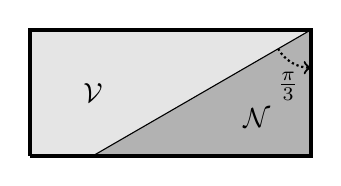
\begin{tikzpicture}[scale=1.6]
\fill [fill=gray!20,draw=black] (2.73,1)--(0.5,1)--(0.5,0)--(1,0);
\fill [fill=gray!60,draw=black] (1,0)--(2.73,0)--(2.73,1)--(1,0);
\draw [ultra thick] (0.5,0)--(2.73,0)--(2.73,1)--(0.5,1)--(0.5,0);
\node[text=black] (n1) at (1,0.5) {$\calV$};
\node[text=black] (n1) at (2.3,0.3) {$\calN$};
\node[text=black] (n1) at (2.55,0.55) {$\frac{\pi}{3}$};
\begin{scope}[shift={(2.73,1)}]
\draw[->,thick,densely dotted] (-150:0.3) arc (-150:-90:0.3);
\end{scope}
\end{tikzpicture}
\\
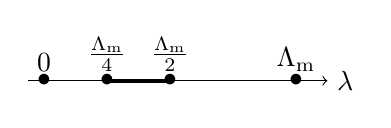
\begin{tikzpicture}[scale=0.4]
\draw [->=latex] (-0.5,0) -> (9,0);
\draw [ultra thick] (2,0) -- (4,0);
\draw (0,0) node {$\bullet$} node[above] {$0$};
\draw (8,0) node {$\bullet$} node[above] {$\Lm$};
\draw (4,0) node {$\bullet$} node[above] {$\frac{\Lm}{2}$};
\draw (2,0) node {$\bullet$} node[above] {$\frac{ \Lm}{4}$};
\draw (9,0) node[right] {$\lambda$};
\end{tikzpicture} &
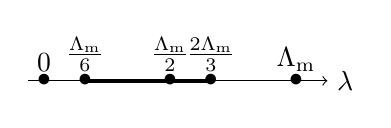
\begin{tikzpicture}[scale=0.4]
\draw [->=latex] (-0.5,0) -> (9,0);
\draw [ultra thick] (1.3,0) -- (5.3,0);
\draw (0,0) node {$\bullet$} node[above] {$0$};
\draw (8,0) node {$\bullet$} node[above] {$\Lm$};
\draw (4,0) node {$\bullet$} node[above] {$\frac{\Lm}{2}$};
\draw [black] (1.3,0) node {$\bullet$} node[above] {$\frac{\Lm}{6}$};
\draw [black] (5.3,0) node {$\bullet$} node[above] {$\frac{2 \Lm}{3}$};
\draw (9,0) node[right] {$\lambda$};
\end{tikzpicture}
\vspace{2mm}
\\
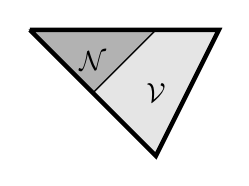
\begin{tikzpicture}[scale=0.4]
\fill [fill=gray!20,draw=black] (2,2)--(4,0)--(6,4)--(4,4)--(2,2);
\fill [fill=gray!60,draw=black] (2,2)--(4,4)--(0,4)--(2,2);
\draw [ultra thick] (0,4)--(4,0)--(6,4)--(0,4);
\node[text=black] (n1) at (2,3) {$\calN$};
\node[text=black] (n1) at (4,2) {$\calV$};
\end{tikzpicture} &
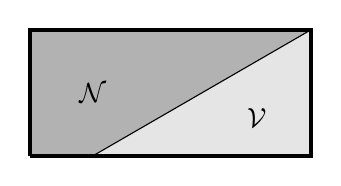
\begin{tikzpicture}[scale=1.6]
\fill [fill=gray!60,draw=black] (2.73,1)--(0.5,1)--(0.5,0)--(1,0);
\fill [fill=gray!20,draw=black] (1,0)--(2.73,0)--(2.73,1)--(1,0);
\draw [ultra thick] (0.5,0)--(2.73,0)--(2.73,1)--(0.5,1)--(0.5,0);
\node[text=black] (n1) at (1,0.5) {$\calN$};
\node[text=black] (n1) at (2.3,0.3) {$\calV$};
\end{tikzpicture}
\\
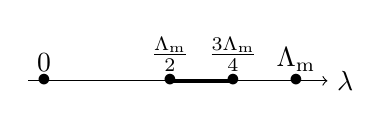
\begin{tikzpicture}[scale=0.4]
\draw [->=latex] (-0.5,0) -> (9,0);
\draw [ultra thick] (6,0) -- (4,0);
\draw (0,0) node {$\bullet$} node[above] {$0$};
\draw (8,0) node {$\bullet$} node[above] {$\Lm$};
\draw (4,0) node {$\bullet$} node[above] {$\frac{\Lm}{2}$};
\draw (6,0) node {$\bullet$} node[above] {$\frac{3 \Lm}{4}$};
\draw (9,0) node[right] {$\lambda$};
\end{tikzpicture} &
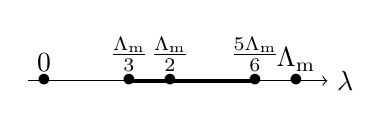
\begin{tikzpicture}[scale=0.4]
\draw [->=latex] (-0.5,0) -> (9,0);
\draw [ultra thick] (2.7,0) -- (6.7,0);
\draw (0,0) node {$\bullet$} node[above] {$0$};
\draw (8,0) node {$\bullet$} node[above] {$\Lm$};
\draw (4,0) node {$\bullet$} node[above] {$\frac{\Lm}{2}$};
\draw (2.7,0) node {$\bullet$} node[above] {$\frac{\Lm}{3}$};
\draw (6.7,0) node {$\bullet$} node[above] {$\frac{5 \Lm}{6}$};
\draw (9,0) node[right] {$\lambda$};
\end{tikzpicture}
\end{tabular}
\end{center}
\caption{Examples of cavities leading to an essential spectrum which is not symmetric with respect to $\Lm/2$. In each column, the domains filled by the Drude material and vacuum are interchanged.}\label{ex2}
\end{figure}

Figures~\ref{ex1} and~\ref{ex2} show various examples which illustrate this theorem.

In Figure~\ref{ex1}, each cavity has an essential spectrum which is symmetric with respect to $\Lm/2$. This clearly holds if there is no boundary vertex $B_q$ (that is, if $\Sigma \cap \partial\calC = \emptyset),$ since the sets $\calJ_p$ are symmetric. This is shown in the left column where we notice that the essential spectrum remains unchanged if we interchange both media, since $\calJ_p$ is unchanged if $\alpha_p$ is replaced by $2\pi - \alpha_p.$ The middle column highlights the fact that $\calI_q = \emptyset$ if $\beta_q = \gamma_q/2$, that is, if the angles of both Drude and vacuum sectors at a boundary vertex $B_q$ are equal. Finally, the right column illustrates the fact that $\calI_q$ is equal to one of the two intervals which compose $\calJ_p$ if $2\beta_q/\gamma_q = \alpha_p/\pi$. Hence, two very different cavities may have the same essential spectrum.

Figure~\ref{ex2} shows examples of cavities leading to an essential spectrum which is no longer symmetric with respect to $\Lm/2$. We notice that if we interchange both media, the new essential spectrum is simply deduced from the initial one by a symmetry with respect to $\Lm/2$, which holds true for all cavities considered here.


\section{Exploration of the spectrum}\label{s-investigation}

\subsection{Preliminaries}\label{s-prelimin}

We first consider the two particular values $\lambda = 0$ and $\lambda = \Lm,$ which are poles of $\epsl_\lambda^\calN$ and $(\mu_\lambda^\calN)^{-1}$ respectively (see~\eqref{e.Drude-model}). The following proposition tells us that $0$ is not an eigenvalue of $\bbA,$ whereas $\Lm$ is an \emph{eigenvalue of infinite multiplicity} of $\bbA.$

\begin{prop}\label{p.partic-values}
We have $\Ker \bbA = \{0\}$ and $\Ker(\bbA - \Lm\Ident) = \calH_\infty \oplus \calH_0$ where $\calH_\infty := \big\{(0,u) \in \calH;\ \Div u = 0 \text{ in }\calN \text{ and } u \cdot n = 0 \text{ on }\Sigma \big\}$ is of infinite dimension whereas $\calH_0$ is a finite dimensional subspace of $\calH.$
\end{prop}

\begin{proof}
Suppose that $(\varphi,u) \in \Ker \bbA,$ which means that $(\varphi,u) \in \rmD(\bbA)$ satisfies~\eqref{e.Lin-one} and~\eqref{e.Lin-two} with $\lambda=0$. Equation~\eqref{e.Lin-two} shows that $u = - \calR \grad \varphi$, so that~\eqref{e.Lin-one} becomes
\[
\frac{1}{\varepsilon_0 \mu_0} \Div (\Un_\calV \grad \varphi) = \Le \Un_\calN \varphi
\quad\text{in }\calC.
\]
The left-hand side of this equation vanishes in $\calN$, therefore $\varphi=0$ in $\calN,$ which implies that $u=0.$ Moreover, this equation shows that $\Delta \varphi=0$ in $\calV$. The trace of $\varphi$ vanishes on $\partial \calV \cap \partial \calC$ (since $\varphi \in H_0^1(\calC))$ as well as on $\Sigma$ (since $\varphi$ is continuous across $\Sigma$, see~\eqref{e.transm.NV}), which implies that $\varphi=0$ in $\calV.$ We conclude that $(\varphi,u)=(0,0)$.

Suppose now that $(\varphi,u) \in \Ker(\bbA - \Lm\Ident),$ which means that $(\varphi,u) \in \rmD(\bbA)$ satisfies~\eqref{e.Lin-one} and~\eqref{e.Lin-two} with $\lambda=\Lm,$ that is,
\begin{align*}
\frac{-1}{\epsl_0 \mu_0}\,\Div \left\{ \grad\varphi + \calR^* u \right\} + (\Un_\calN\,\Le - \Lm)\,\varphi &= 0 \quad\text{in }\calC, \\
\calR\grad\varphi &= 0 \quad\text{in }\calN.
\end{align*}
\goodbreak

\begingroup
The latter equation implies that $\varphi$ is constant in $\calN.$ Assuming for simplicity that $\partial\calN \cap \partial\calC \neq \emptyset,$ this constant must vanish (since $\varphi|_{\partial\calC} = 0),$ so the former equation shows on the one hand that $\varphi_\calV := \varphi|_\calV$ is a solution in $H^1_0(\calV)$ to
\[
-\Delta \varphi_\calV - \epsl_0 \mu_0 \Lm\,\varphi_\calV = 0 \quad\text{in }\calV,
\]
and on the other hand that $u$ satisfies
\[
\Div u = 0 \text{ in }\calN
\quad\text{and}\quad u \cdot n = \frac{\partial\varphi_\calV}{\partial n}\text{ on }\Sigma.
\]
\endgroup
If $\epsl_0 \mu_0 \Lm$ is not an eigenvalue of the Dirichlet Laplacian in $\calV,$ we conclude that $\varphi_\calV = 0.$ This shows that $\Ker(\bbA - \Lm\Ident)$ coincide in this case with the subspace $\calH_\infty$ defined in the Proposition~\ref{p.partic-values}, whose dimension is clearly infinite since it contains all pairs $(0,\curl\psi)$ where $\psi \in H^1(\calN)$ satisfies $\psi|_\Sigma =0$ (here, $\curl$ denotes the two-dimensional curl of a scalar function, i.e., $\curl\psi := (\partial\psi/\partial y, -\partial\psi/\partial x).$

But if by chance, $\epsl_0 \mu_0 \Lm$ is an eigenvalue of the Dirichlet Laplacian in $\calV,$ then $\varphi_\calV$ can be any associated eigenfunction, which yields element $(\phi,u) \in \Ker(\bbA - \Lm\Ident)$ with $\phi \neq 0.$ Hence in this case, $\Ker(\bbA - \Lm\Ident)$ does not reduce to $\calH_\infty,$ but the orthogonal complement of $\calH_\infty$ in $\Ker(\bbA - \Lm\Ident)$ has necessarily a finite dimension since the eigenvalues of the Dirichlet Laplacian have a finite multiplicity.

The above arguments are easily adapted if $\partial\calN \cap \partial\calC = \emptyset.$
\end{proof}

\begin{rema}\label{r-artifact}
The above Proposition~\ref{p.partic-values} shows that the fact that $\Lm$ belongs to the essential spectrum of $\bbA$ is related to the infinite dimensional subspace $\calH_\infty.$ The eigenfunctions $(\varphi,u)$ of this subspace are such that $\varphi = 0.$ Hence these states cannot be revealed by the nonlinear eigenvalue problem~\eqref{e.NLin}. This is why $\Lm$ can be seen as an artifact of the augmented formulation~\eqref{e.Lin}.
\end{rema}


\subsection{Bulk resonance in the Drude material}\label{s-bulk-reson}

As mentioned in Section~\ref{s-main-results}, each point of the essential spectrum of $\bbA$ (except $\Lm)$ is related to an unusual resonance phenomenon. The case of $\lambda = 0$ is related to the existence at low frequencies of highly oscillating vibrations which are confined in the Drude material. Assuming $\partial\calV \cap \partial\calC \neq \emptyset$ (which is not necessary in Proposition~\ref{p-Weyl-bulk} below), this can be understood intuitively from~\eqref{e.Helm.N}--\eqref{e.Diri} by first noticing that in the second transmission condition of~\eqref{e.transm.NV}, $\frac{1}{\mu_\lambda^\calN}$ tends to $0$ when $\lambda$ tends to $0$, which shows that on the vacuum side, the normal derivative of $\varphi$ must be small. Hence, in the vacuum, $\varphi$ is close to a solution to the Helmholtz equation~\eqref{e.Helm.V} which vanishes on $\partial\calV \cap \partial\calC$ and such that $\partial\varphi/\partial n = 0$ on $\Sigma.$ The eigenvalues $\lambda$ of this problem are positive (thanks to the assumption $\partial\calV \cap \partial\calC \neq \emptyset$), so the only possible solution for small $\lambda$ is $\varphi|_\calV = 0$, which means that $\varphi$ is confined in $\calN.$ Besides, we have seen in Section~\ref{s-nonlinear} that in a cavity which only contains a Drude material, eigenvalues accumulate at 0. This gives the idea of the construction of a Weyl sequence for $\lambda = 0.$

Consider a sequence $(\varphi_n^\calN)$ of eigenfunctions of the Dirichlet Laplacian in $\calN,$ i.e., a sequence of nonzero solutions $\varphi_n^\calN \in H^1_0(\calN)$ to $-\Delta \varphi_n^\calN = \lambda_n \varphi_n^\calN,$ where $(\lambda_n)$ is the sequence of associated eigenvalues, which tends to $+\infty.$ The idea is simply to extend $\varphi_n^\calN$ by 0 in $\calV$ and introduce the corresponding auxiliary unknown defined by~\eqref{e.def-u} with $\lambda=0.$
\pagebreak


\begin{prop}\label{p-Weyl-bulk}
Let $\Phi_n := (\varphi_n,u_n)$ where $\varphi_n := \calR^* \varphi_n^\calN$ and $u_n :=\linebreak- \calR \grad \varphi_n.$ Then $\Phi_n/\|\Phi_n\|_\calH$ is a Weyl sequence for $\lambda = 0.$
\end{prop}


\begin{proof}
As $\varphi_n^\calN \in H_0^1(\calN)$, we have $\grad (\calR^* \varphi_n^\calN) = \calR^* \grad \varphi_n^\calN,$ so $\varphi_n \in H_0^1(\calC)$ and $u_n = - \grad \varphi_n^\calN \in L^2(\calN)$. Moreover, $\Div (\grad \varphi_n + \calR^* u_n) = 0,$ which shows that $\Phi_n \in \rmD(\bbA)$ (see~\eqref{e.def-Dom-A}).

Besides, from the definition~\eqref{e.defA} of $\bbA,$ we see that $\bbA \Phi_n = (\Un_\calN \Le \, \varphi_n,0)$, so
\[
\frac{\| \bbA \Phi_n \|_\calH}{\| \Phi_n \|_\calH}
\lesssim \frac{ \| \varphi_n^\calN \|_{L^2(\calN)} }{\| u_n \|_{L^2(\calN)}} = \frac{ \| \varphi_n^\calN \|_{L^2(\calN)} }{\| \grad \varphi_n^\calN \|_{L^2(\calN)}} = \frac{1}{\sqrt{\lambda_n}},
\]
where the last equality follows from the definition of $\varphi_n^\calN.$ As $\lambda_n \to +\infty$, we deduce that $0$ is in the spectrum of operator $\bbA$.

It is not necessary here to check the weak convergence to 0 of $\Phi_n/\|\Phi_n\|_\calH.$ Indeed, Proposition~\ref{p.partic-values} tells us that $0$ is not an eigenvalue of $\bbA,$ so it belongs necessarily to its essential spectrum.
\end{proof}

We show in the next Subsections~\ref{s-surface-reson}--\ref{s.proof-thm} that the other components of the essential spectrum of $\bbA$ are located outside a vicinity of $0.$ In other words, $0$ is an isolated point of $\sigma_{\ess}(\bbA).$ Therefore, as it is not an eigenvalue, $0$ \emph{is an accumulation point of} $\sigma_{\disc}(\bbA),$ as in the case $\calV = \emptyset$ mentioned in Section~\ref{s-nonlinear}. The following Proposition~\ref{prop3.4} confirms the initial intuitive assertion of this subsection: the eigenfunctions associated to eigenvalues close to 0 are actually confined in the Drude material.

\begin{prop}\label{prop3.4}
Assume that $\partial\calV \cap \partial\calC \neq \emptyset.$ Let $(\lambda_j)_{j \in \bbN}$ be a sequence of $\sigma_{\disc}(\bbA)$ which tends to $0$ and $\Phi_j = (\varphi_j,u_j)$ a sequence of associated eigenvectors chosen such that $\| \Phi_j \|_\calH = 1.$ Then the restrictions $\varphi_j|_\calV$ tend to $0$ in $H^1(\calV).$
\end{prop}

\begin{proof}
In Section~\ref{s-linear}, we have seen that the linear eigenvalue equation $A \Phi_j\linebreak= \lambda_j\,\Phi_j$ is equivalent to the initial nonlinear one
\[
\Div \left(\frac{1}{\mu_{\lambda_j}}\, \grad\varphi_j \right) + \lambda_j\,\epsl_{\lambda_j}\,\varphi_j = 0
\quad\text{in }\calC,
\]
together with $u_j = \Lm \, (\lambda_j-\Lm)^{-1} \, \calR \grad\varphi_j.$ Using Green's formula, we deduce from the above equation that
\[
\int_\calC \left(\frac{1}{\mu_{\lambda_j}}\, |\grad\varphi_j|^2 - \lambda_j\,\epsl_{\lambda_j}\,|\varphi_j|^2 \right) \rmd x = 0.
\]
Splitting the integral in two parts on $\calV$ and $\calN$ and gathering the terms with same sign yields
\[
\frac{1}{\mu_0}\,\int_\calV |\grad\varphi_j|^2 \,\rmd x +
\lambda_j\,|\epsl^\calN_{\lambda_j}| \,\int_\calN |\varphi_j|^2 \,\rmd x = \frac{1}{|\mu^\calN_{\lambda_j}|}\,\int_\calN |\grad\varphi_j|^2 \,\rmd x +
\lambda_j\,\epsl_0 \,\int_\calV |\varphi_j|^2 \,\rmd x.
\]
The right-hand side of this equality tends to 0, for both integrals are bounded (since $\| \Phi_j \|_\calH = 1)$ and both factors $1/\mu^\calN_{\lambda_j}$ and $\lambda_j$ tend to 0. Therefore the left-hand side also tends to 0, which implies that $\grad\varphi_j|_\calV \to 0$ in $L^2(\calV).$ Thanks to the assumption $\partial\calV \cap \partial\calC \neq \emptyset,$ Poincaré's inequality then shows that $\varphi_j|_\calV$ tend to $0$ in $H^1(\calV).$
\end{proof}

\subsection{Surface resonance at the interface between both media}\label{s-surface-reson}
We prove now that $\lambda = \Lm/2$ also belongs to the essential spectrum. This value corresponds to the case where $\mu_\lambda^\calN = -\mu_0,$ that is, the critical value $-1$ of the contrast $\mu_\lambda^\calN/\mu_0$, which is known to lead to an ill-posed time-harmonic problem (see the references quoted in the introduction). As shown below, it is related to the existence of highly oscillating vibrations that can be localized near any point of the interface $\Sigma$ except the vertices. We first show how such \emph{surface waves} can be derived from our initial equation~\eqref{e.NLin}.


\begin{figure}[!t]
\begin{center}
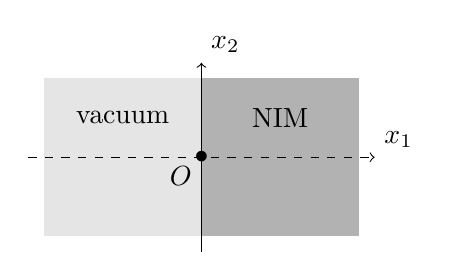
\begin{tikzpicture}
\fill[fill=gray!20] (-2,-1) rectangle (0,1);
\fill[fill=gray!60] (0,-1) rectangle (2,1);
\draw [->=latex,dashed] (-2.2,0)--(2.2,0);
\draw [->=latex] (0,-1.2)--(0,1.2);
\draw (2.2,0) node[above right] {$x_1$};
\draw (0,1.2) node[above right] {$x_2$};
\draw (0,0) node {$\bullet$} node[below left] {$O$};
\draw (-1,0.5) node {vacuum};
\draw (1,0.5) node {NIM};
\end{tikzpicture}
\end{center}
\caption{Cartesian coordinates near a point of the interface $\Sigma.$}\label{f.surf-res}
\end{figure}

\subsubsection{Surface waves}
Consider the case of a rectilinear interface between two half-planes. Choose a Cartesian coordinate system $(O,x_1,x_2)$ so that the half-plane $x_1 > 0$ is filled by our NIM, whereas $x_1 < 0$ contains vacuum (see Figure~\ref{f.surf-res}). Consider then the equation
\begin{equation}\label{e.NLin.appr}
\Div \left(\frac{1}{\mu_{\Lm/2}} \grad \psi \right) = 0,
\end{equation}
which is deduced from~\eqref{e.NLin} with $\lambda = \Lm/2$ by removing the term $\lambda\,\epsl_\lambda\,\varphi$ (as shown in the following, this term acts as a ``small'' perturbation for highly oscillating solutions). It is readily seen that for any $k>0$, the function $\exp(\rmi k(x_2 + \rmi |x_1|)$ is a solution to~\eqref{e.NLin.appr}. It represents a surface wave which propagates in the direction of the interface and decreases exponentially as $x_1 \to \pm\infty.$ Any superposition of such surface waves (for various $k)$ is still solution to~\eqref{e.NLin.appr}. In particular, for a given $f \in \calD(\bbR^+),$ the function $\psi$ defined by
\[
\psi(x) = \psi(x_1,x_2) :=
\int_{\bbR^+} f(k)\,\rme^{\rmi k(x_2 + \rmi |x_1|)}\, \rmd k
\]
is a solution to~\eqref{e.NLin.appr}, as well as
\[
\psi_n(x) := \psi(nx_1,nx_2) =
\int_{\bbR^+} \frac{1}{n}\,f\left(\frac{k}{n}\right)\,\rme^{\rmi k(x_2 + \rmi |x_1|)}\, \rmd k
\quad\text{for }n \geq 1.
\]

\begin{rema}\label{r.surf-res}
By successive integrations par parts, we see that $\psi(x) = o(|x|^{-p})$ for all $p \in \bbN$ as $|x| := \sqrt{x_1^2 + x_2^2}$ goes to $+\infty,$ and the same holds for the first-order partial derivatives of $\psi$ (note that $\partial\psi/\partial x_1$ is discontinuous across $x_1=0).$ This shows in particular that $\psi \in H^1(\bbR^2).$ Hence $\psi$ represents vibrations which are localized in a bounded region near the interface, whereas $\psi_n$ becomes more and more confined near $O$ as $n$ increases. Notice that $\psi$ (as well as $\psi_n)$ is symmetric with respect to $x_1=0,$ that is, $\psi(-x_1,x_2) = \psi(x_1,x_2).$
\end{rema}

\subsubsection{A Weyl sequence}
Returning to our cavity, we are now able to construct a Weyl sequence for\linebreak$\lambda = \Lm/2$. Suppose that the center $O$ of our coordinate system $(O,x_1,x_2)$ is a given point of the interface $\Sigma$ different from the vertices and that the $x_1$ and $x_2$-axes are chosen such that our medium is described by Figure~\ref{f.surf-res} in a vicinity of $O.$ More precisely, this means that one can choose a given small enough $R>0$ such that $B_R \subset \calC,$ $\calN \cap B_R \subset \{x_1 > 0\}$ and $\calV \cap B_R \subset \{x_1 < 0\},$ where we have denoted $B_R := \{ x \in \bbR^2;\ |x| \le R \}$ the ball of radius $R$ centered at $O.$ Let us then define
\begin{equation}\label{e.Weyl-seq-surf}
\varphi_n := \psi_n \ \chi
\quad\text{and}\quad u_n := -2 \calR \grad \varphi_n,
\end{equation}
where $\chi \in \calD(\bbR^2)$ is a cutoff function which vanishes outside $B_R,$ is equal to 1 in some ball $B_{R_1}$ with $0 < R_1 < R$ and is symmetric with respect to $x_1=0,$ that is, $\chi(-x_1,x_2) = \chi(x_1,x_2).$ Note that the above definition of $u_n$ follows from~\eqref{e.def-u} with $\lambda=\Lm/2$.

\begin{prop}\label{p-Weyl-surface}
Let $\Phi_n := (\varphi_n,u_n)$ defined by~\eqref{e.Weyl-seq-surf}. Then $\Phi_n/\|\Phi_n\|_\calH$ is a Weyl sequence for $\lambda = \Lm/2$.
\end{prop}

\begin{proofc}
\begin{step}\label{proofprop3.6.1}
Let us first prove that $\Phi_n \in \rmD(\bbA)$. It is clear that $\psi_n$ is a $\calC^\infty$ function in both half-planes $\pm x_1 > 0$ and is continuous at the interface $x_1 = 0.$ Hence $\varphi_n \in H_0^1(\calC)$ (since $\chi=0$ on $\partial \calC)$, which implies that $u_n \in L^2(\calN)^2$. It remains to check that $\Div(\grad \varphi_n + \calR^* u_n) = - \Div (s_1 \, \grad \varphi_n)$ belongs to $L^2(\calC),$ where $s_1$ denotes the sign function $s_1(x_1,x_2) := \sgn x_1.$ As $\varphi_n$ is smooth on both sides of the interface, this amounts to proving that $s_1 \, \partial \varphi_n/\partial x_1$ is continuous across the interface. We have
\[
\frac{\partial \varphi_n}{\partial x_1} = \psi_n \,\frac{\partial \chi}{\partial x_1} + \frac{\partial \psi_n}{\partial x_1}\,\chi.
\]
As $\chi \in \calD(\bbR^2)$ is symmetric with respect to $x_1=0,$ its partial derivative $\partial \chi/\partial x_1$ vanishes on the interface. On the other hand, $\psi_n$ is continuous but not differentiable on the interface. However it is symmetric with respect to $x_1=0,$ so that $s_1 \, \partial \psi_n/\partial x_1$ is continuous across the interface, which yields the desired result.
\end{step}

\begin{step}\label{proofprop3.6.2}
We prove now that $\|\bbA \Phi_n - (\Lm/2)\,\Phi_n\|_\calH/\|\Phi_n\|_\calH$ tends to $0$ as $n \to \infty$. First, using the fact that $\psi_n$ is solution to~\eqref{e.NLin.appr} where $\mu_{\Lm/2} = -s_1\,\mu_0,$ we infer that
\[
\bbA \Phi_n - \frac{\Lm}{2}\, \Phi_n =
\begin{pmatrix}
\displaystyle\frac{s_1}{\varepsilon_0 \mu_0}
\Big(2 \grad\psi_n \cdot \grad\chi + \psi_n\,\Delta \chi \Big) + \left(\Un_\calN \Le - \frac{\Lm}{2} \right) \psi_n\,\chi \\
0
\end{pmatrix}.
\]

As $\grad\chi$ and $\Delta \chi$ vanish outside $B_R \setminus B_{R_1},$ we deduce
\[
\left\| \bbA \Phi_n - \frac{\Lm}{2}\, \Phi_n \right\|_\calH
\lesssim
\big\| \psi_n \big\|_{H^1(B_R \setminus B_{R_1})} + \big\| \psi_n \big\|_{L^2(B_R)}.
\]
Both terms of the right-hand side tend to $0$ as $n \to \infty,$ which follows from the fact that $\psi \in H^1(\bbR^2)$ (see Remark~\ref{r.surf-res}). Indeed, by a simple change of variable $nx \mapsto x,$ we have on the one hand,
\begin{equation}\label{e.psi-n}
\big\| \psi_n \big\|_{L^2(B_R)}^2 = \int_{B_R} |\psi(nx)|^2\,\rmd x = \frac{1}{n^2}\, \int_{B_{nR}} |\psi(x)|^2\,\rmd x
\leq \frac{1}{n^2}\, \big\| \psi \big\|_{L^2(\bbR^2)}^2
\to 0
\end{equation}
and on the other hand, for $j=1,2,$
\begin{equation}\label{e.dpsi-n}
\left\| \frac{\partial \psi_n}{\partial x_j}\right\|_{L^2(B_R \setminus B_{R_1})}^2 = \int_{B_{nR} \setminus B_{nR_1}} \left| \frac{\partial \psi}{\partial x_j} (x) \right|^2 \,\rmd x
\leq \left\| \frac{\partial \psi}{\partial x_j}\right\|_{L^2(\bbR^2 \setminus B_{nR_1})}^2
\to 0.
\end{equation}

It remains to check that $\| \Phi_n \|_\calH \gtrsim 1.$ First notice that
\[
\| \Phi_n \|_\calH
\gtrsim \|u_n\|_{L^2(\calN)^2}
\gtrsim \left\| \frac{\partial \varphi_n}{\partial x_1} \right\|_{L^2(\calN)}
\geq \left\| \frac{\partial \psi_n}{\partial x_1}\, \chi \right\|_{L^2(\calN)} - \left\| \psi_n\, \frac{\partial \chi}{\partial x_1} \right\|_{L^2(\calN)}.
\]
As $\chi = 1$ in $B_{R_1}$ and $\chi = 0$ outside $B_R,$ we infer that
\[
\| \Phi_n \|_\calH
\gtrsim \left\| \frac{\partial \psi_n}{\partial x_1} \right\|_{L^2(B_{R_1}^+)} - \left\| \psi_n \right\|_{L^2(B_R^+)}
\,\left\| \frac{\partial \chi}{\partial x_1} \right\|_{L^2(B_R^+)},
\]
where we have denoted $B_R^+ := B_R \cap \calN.$ We know from~\eqref{e.psi-n} that $\| \psi_n \|_{L^2(B_R)}$ tends to $0,$ thus so does $\| \psi_n \|_{L^2(B_R^+)}$. Moreover, similarly as in~\eqref{e.dpsi-n}, we have
\[
\left\| \frac{\partial \psi_n}{\partial x_1}\right\|_{L^2(B_{R_1}^+)}^2 = \int_{B_{nR_1}^+} \left| \frac{\partial \psi}{\partial x_1} (x) \right|^2 \,\rmd x
\longrightarrow \left\| \frac{\partial \psi}{\partial x_1}\right\|_{L^2(\bbR^+ \times \bbR)}^2 > 0
\quad\text{as } n \to \infty.
\]
We conclude that $\| \Phi_n \|_\calH \gtrsim 1$ for large enough $n$, so 
\[
\frac{\| \bbA \Phi_n - (\Lm/2)\,\Phi_n\|_\calH}{\| \Phi_n\|_\calH}
\;\to 0\;\text{ as } n \to \infty.
\] 
\end{step}


\begin{step}\label{proofprop3.6.3}
Lastly, we prove that $\Phi_n$ converges weakly to 0 as $n \to \infty$ (so the same holds true for $\Phi_n/\|\Phi_n\|_\calH$ since $\| \Phi_n \|_\calH \gtrsim 1).$ For any given $\Phi' := (\varphi',u') \in \calD(\calC) \times \calD(\calN)^2,$ we have
\[
\Big| (\Phi_n,\Phi')_\calH \Big|
\lesssim
\int_{B_R} \left(\big| \psi(nx) \big| + n \big| \grad\psi(nx) \big| \right) \rmd x.
\]
So, using again the change of variable $nx \to x,$ we deduce that
\[
\Big| (\Phi_n,\Phi')_\calH \Big|
\lesssim
\int_{B_{nR}} \left(\frac{1}{n^2}\,\big| \psi(x) \big| + \frac{1}{n}\,\big| \grad\psi(x) \big| \right) \rmd x.
\]
As $\psi(x) = o(|x|^{-p})$ and $\grad \psi(x) = o(|x|^{-p})$ for all $p \in \bbN$ as $|x|\to +\infty$ (see Remark~\ref{r.surf-res}), we infer that $\psi$ and both components of $\grad \psi$ belong to $L^1(\bbR^2).$ The conclusion follows.
\end{step}
\end{proofc}

\subsection{Corner resonance at an inner vertex}\label{s-inner-vertex}
It remains to deal with the intervals of essential spectrum $\calJ_p$ and $\calI_q$ defined in Section~\ref{s-main-results}, associated respectively with the inner and boundary vertices of the interface $\Sigma$ between $\calN$ and $\calV.$ In this subsection, we consider the case of an inner vertex $C_p$ near which the NIM fills a sector of angle $\alpha_p \in (0,2\pi)$ (see Figure~\ref{f.cavity}). The next Subsection~\ref{s-bound-vertex} is devoted to boundary vertices.

\subsubsection{Black hole waves}\label{subsub3.4.1}


\begin{figure}
\begin{center}
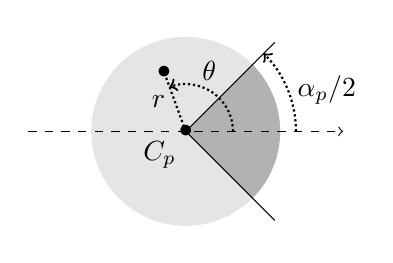
\begin{tikzpicture}[scale=0.4]
\fill[fill=gray!20] (0,0) -- (45:3) arc (45:315:3);
\fill[fill=gray!60] (0,0) -- (-45:3) arc (-45:45:3);
\draw[->=latex, dashed] (-5,0) -- (5,0);
\draw (0,0) node{$\bullet$} node[below left] {$C_p$};
\draw (110:2) node{$\bullet$};
\draw[->,thick,densely dotted] (0:1.5) arc (0:110:1.5);
\draw[thick,densely dotted] (0,0) -- (110:2);
\draw (60:1.5) node[above] {$\theta$};
\draw (110:1) node[left] {$r$};
\draw (0,0) -- (45:4);
\draw (0,0) -- (-45:4);
\draw[->,thick,densely dotted] (0:3.5) arc (0:45:3.5);
\draw (22:3.5) node[right] {$\alpha_p/2$};
\end{tikzpicture}
\hspace{1cm}
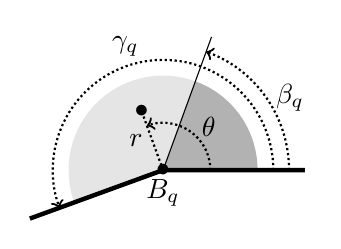
\begin{tikzpicture}[scale=0.4]
\fill[fill=gray!60] (0,0) -- (0:3) arc (0:70:3);
\fill[fill=gray!20] (0,0) -- (70:3) arc (70:200:3);
\draw[->,thick,densely dotted] (0:1.5) arc (0:110:1.5);
\draw[->,thick,densely dotted] (0:4) arc (0:70:4);
\draw[->,thick,densely dotted] (0:3.5) arc (0:200:3.5);
\draw [ultra thick] (0:4.5) -- (0,0) -- (200:4.5);
\draw[thick,densely dotted] (0,0) -- (110:2);
\draw (0,0) -- (70:4.5);
\draw (110:2) node{$\bullet$};
\draw (110:1) node[left] {$r$};
\draw (40:1.2) node[above right] {$\theta$};
\draw (35:4) node[right] {$\beta_q$};
\draw (110:3.5) node[above] {$\gamma_q$};
\draw (0,0) node{$\bullet$} node[below] {$B_q$};
\end{tikzpicture}
\end{center}
\caption{Polar coordinates near an inner vertex $C_p$ (left) and near a boundary vertex $B_q$ (right).}\label{f.polar-coord}
\end{figure}

The part of the essential spectrum that we study here is related to the existence of highly oscillating vibrations localized near $C_p,$ which have been interpreted as a ``black hole'' phenomenon in~\cite{Bon-etal-16}. We first recall the construction of the so-called \emph{black hole waves}, first introduced in~\cite{Bon-Dau-Ram-99}. As in Section~\ref{s-surface-reson}, we are interested in solutions to
\begin{equation}\label{e.eq-black-hole}
\Div(\mu_\lambda^{-1} \grad \psi_\lambda) = 0 \quad\text{in the whole plane }\bbR^2,
\end{equation}
but instead of a plane interface, we suppose now that the two sectors of NIM and vacuum defined near $C_p$ are extended up to infinity. More precisely, by choosing polar coordinates $(r, \theta) \in \bbR^+ \times (-\pi,+\pi]$ centered at $C_p$ and such that the Drude sector corresponds to $|\theta| < \alpha_p/2$ (see Figure~\ref{f.polar-coord}, left), this equation writes equivalently as
\[
r \, \frac{\partial}{\partial r} \left(r \frac{\partial \psi_\lambda}{\partial r} \right) + \mu_\lambda \, \frac{\partial }{\partial \theta} \left(\frac{1}{\mu_\lambda} \frac{\partial \psi_\lambda}{\partial \theta} \right) = 0
\]
where $\mu_\lambda = \mu_\lambda(\theta)$ is defined by $\mu_\lambda(\theta) = \mu_\lambda^\calN$ if $|\theta| < \alpha_p/2$ and $\mu_\lambda(\theta) = \mu_0$ if $|\theta| > \alpha_p/2$. In this situation, we can use the technique of separation of variables (which would have not been possible without removing the term $\lambda\,\epsl_\lambda\,\varphi$ in~\eqref{e.NLin}), which yields
\begin{equation}
\psi_\lambda(r,\theta) = r^{\rmi\eta_\lambda}\ m_\lambda(\theta),\label{e.def-psi-lambda}
\end{equation}
where $\eta_\lambda$ is a complex parameter and the angular modulation $m_\lambda$ is a $2\pi$-periodic solution to
\begin{equation}
\mu_\lambda \, \frac{\rmd}{\rmd \theta} \left(\frac{1}{\mu_\lambda} \frac{\rmd m_\lambda}{\rmd \theta} \right) - \eta_\lambda^2 \, m_\lambda = 0
\quad \text{in } (-\pi,+\pi).\label{e.ang-mod}
\end{equation}
It is easily seen that this equation admits a non-trivial solution if and only if $\eta_\lambda$ satisfies the dispersion equation
\begin{equation}\label{e.equa-disp}
\left(\frac{\sinh\big(\eta_\lambda(\pi-\alpha_p)\big)}{\sinh(\eta_\lambda\pi)} \right)^2 =
\left(\frac{\mu_0 + \mu_\lambda^\calN}{\mu_0 - \mu_\lambda^\calN} \right)^2
\quad\text{where}\quad
\frac{\mu_0 + \mu_\lambda^\calN}{\mu_0 - \mu_\lambda^\calN} = \frac{\lambda-\Lm/2}{\Lm/2}.
\end{equation}


We are actually interested in \emph{real solutions} $\eta_\lambda$ of this equation. Indeed, in this case, the radial behavior $r^{\rmi\eta_\lambda} = \exp(\rmi\eta_\lambda \log r)$ of $\psi_\lambda$ has a constant amplitude and is increasingly oscillating as $r$ goes to 0. Because of these oscillations, $\grad \psi_\lambda$ is not square-integrable near $C_p$ (indeed $|\partial \psi_\lambda(r,\theta) / \partial r| \gtrsim r^{-1}).$ From a physical point of view, this means that any vicinity of $C_p$ contains an infinite energy. In fact, $\psi_\lambda$ represents a wave which propagates towards the corner and whose energy accumulates near this corner, which explains its interpretation as a \emph{black hole wave}.

Without loss of generality, we can restrict ourselves to positive $\eta_\lambda.$ Noticing that the function
$
(0,+\infty) \ni \eta \mapsto |\sinh\big(\eta(\pi-\alpha_p)\big)/\sinh(\eta\pi)|
$
is strictly decreasing with range $(0,|1 - \alpha_p/\pi|),$ we infer that~\eqref{e.equa-disp} has a unique solution $\eta_\lambda \in (0,+\infty)$ if and only if
\[
0 < \left| \lambda - \frac{\Lm}{2} \right| < \frac{\Lm}{2} \ \left| 1 - \frac{\alpha_p}{\pi}\right|,
\]
which leads to the definition~\eqref{e.def-J_p} of $\calJ_p.$ Moreover, when $\lambda$ varies in one of the two intervals which compose $\calJ_p,$ the solution $\eta_\lambda$ ranges from $+\infty$ (as $\lambda \to \Lm/2)$ to 0 (as $\lambda \to \{ 1 \pm |1-\alpha_p/\pi|\} \,\Lm/2).$

\begin{figure}
\begin{center}
\centering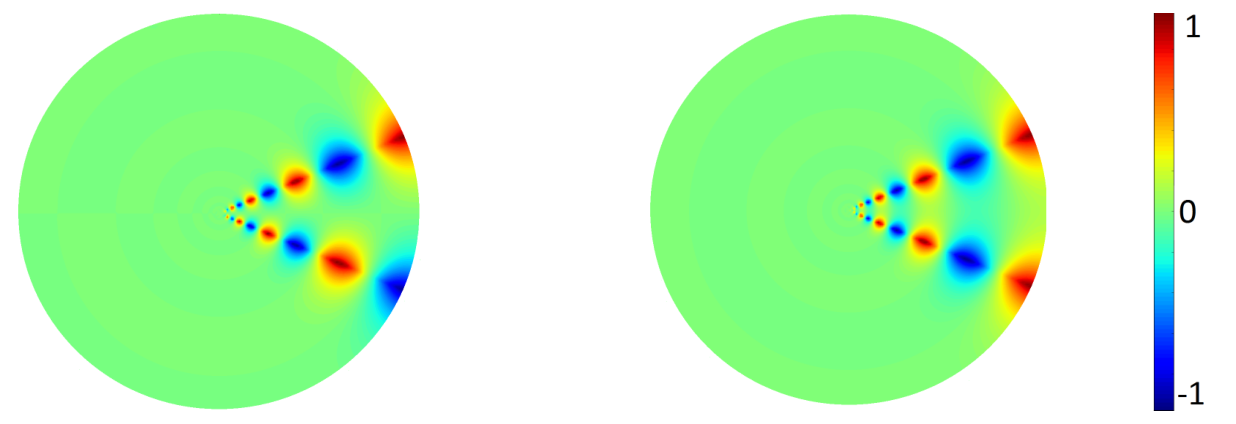
\includegraphics[width=309pt]{../assets/2637/black-hole-wave-visuals.png} 
%\includegraphics[height=3.5cm]{Figures/Blackhole fig-a.pdf}\hspace{2cm}\includegraphics[height=3.95cm]{Figures/Blackhole fig-b.pdf} 
%\includegraphics[height=3.5cm]{black-hole-sh.png}\hspace{2cm}\includegraphics[height=3.5cm]{black-hole-ch.png}
\end{center}
\caption{For $\alpha_p = \pi/4,$ representation of the real part of the black hole wave $r^{\rmi \eta_\lambda}\,m_\lambda(\theta)$ for $\lambda = \Lm /4$ (left, $m_\lambda$ given by~\eqref{e.m_lambda-sh}) and $\lambda = 3\Lm /4$ (right, $m_\lambda$ given by~\eqref{e.m_lambda-ch}).}\label{f.black-hole}
\end{figure}

For a given $\lambda \in \calJ_p,$ the expression of the corresponding solution $m_\lambda$ to~\eqref{e.ang-mod} depends on the respective signs of the quantities inside both squared terms in~\eqref{e.equa-disp}. Two situations occur. On the one hand, if $(\alpha_p < \pi$ and $\lambda < \Lm/2)$ or $(\alpha_p > \pi$ and $\lambda > \Lm/2),$ then the angular modulation $m_\lambda$ is given (up to a complex factor) by
\begin{equation}\label{e.m_lambda-sh}
m_\lambda(\theta) :=
\begin{cases}
\displaystyle
\mkern50mu\frac{\sinh(\eta_\lambda \theta)}{\sinh(\eta_\lambda \frac{\alpha_p}{2})} & \text{if }\displaystyle |\theta| < \frac{\alpha_p}{2}, \\[8pt]
\displaystyle
\frac{\sgn(\theta) \ \sinh\big(\eta_\lambda (\pi - |\theta|)\big)}{\sinh\big(\eta_\lambda (\pi - \frac{\alpha_p}{2})\big)} & \text{if }\displaystyle |\theta| > \frac{\alpha_p}{2}.
\end{cases}
\end{equation}
On the other hand, if $(\alpha_p < \pi$ and $\lambda > \Lm/2)$ or $(\alpha_p > \pi$ and $\lambda < \Lm/2)$, then
\begin{equation}\label{e.m_lambda-ch}
m_\lambda(\theta) := 
\begin{cases}
\displaystyle
\mkern30mu\frac{\cosh(\eta_\lambda \theta)}{\cosh(\eta_\lambda \frac{\alpha_p}{2})} & \text{if }\displaystyle |\theta| < \frac{\alpha_p}{2}, \\[8pt]
\displaystyle
\frac{\cosh\big(\eta_\lambda (\pi - |\theta|)\big)}{\cosh\big(\eta_\lambda (\pi - \frac{\alpha_p}{2})\big)} & \text{if }\displaystyle |\theta| > \frac{\alpha_p}{2}.
\end{cases}
\end{equation}
These formulas are illustrated by Figure~\ref{f.black-hole} which represents the associated black hole wave defined by~\eqref{e.def-psi-lambda} in two particular cases that correspond to the same $\eta_\lambda$. Both figures are very similar: both represent surface waves which propagate along the interfaces and concentrate near the vertex. The main difference is the symmetry or skew-symmetry with respect to the symmetry axis of the corner.

\subsubsection{Weyl sequences}
Black hole waves are the basic ingredients for the construction of Weyl sequences here. As mentioned above, the gradient of $\psi_\lambda$ is not square-integrable near $C_p$ because of its increasingly oscillating behavior. Hence, a natural idea for a Weyl sequence is to truncate $\psi_\lambda$ using a sequence of cutoff functions whose supports get closer and closer to $C_p.$ As shown at the end of this subsection, this is a bad idea! A proper idea to define a Weyl sequence for a given $\lambda_* \in \calJ_p$ consists in considering continuous superpositions of the black hole waves $\psi_\lambda,$ choosing smooth densities of superposition with increasingly small supports near $\lambda_*.$ Such superpositions regularize the behavior of the black hole waves near the corner (thanks to the smoothness of the densities) and resemble more and more $\psi_{\lambda_*}$ (thanks to the increasingly small supports).

From a practical point of view, it is actually more convenient to consider superpositions with respect to the variable $\eta$ (instead of $\lambda)$ near $\eta_* := \eta_{\lambda_*} \in (0,+\infty).$ This leads to introduce the inverse function $\eta \mapsto \lambda(\eta)$ of $\lambda \mapsto \eta_\lambda$ considered in the half part of $\calJ_p$ which contain our given $\lambda_*.$ We deduce from~\eqref{e.equa-disp} that this function is given by
\[
\lambda(\eta) = \frac{\Lm}{2}\ \left(1 + \sgn\left(\lambda_* - \frac{\Lm}{2}\right) \
\frac{\sinh\big(\eta\,|\pi-\alpha_p|\big)}{\sinh(\eta\,\pi)}
\right),
\quad\forall \eta \in (0,+\infty).
\]
Then, for all integer $n \geq 1,$ we define
\begin{equation}\label{e.Weyl-seq-vertex}
\begin{pmatrix} \varphi_n \\ u_n
\end{pmatrix}
:= \chi\,
\begin{pmatrix} \tilde \varphi_n \\ \tilde u_n
\end{pmatrix}
\quad\text{where}\quad
\begin{cases}
\displaystyle \tilde\varphi_n := \int_\bbR f_n(\eta)\, \psi_{\lambda(\eta)} \,\rmd\eta \quad\text{and} \\[10pt]
\displaystyle \tilde u_n := \int_\bbR f_n(\eta)\, \frac{\Lm}{\lambda(\eta)-\Lm}\,\calR \grad\psi_{\lambda(\eta)} \,\rmd\eta,
\end{cases}
\end{equation}
where $\chi$ and $f_n$ are chosen as follows. First choose some $R>0$ such that $\calN \cap B_R$ and $\calV \cap B_R$ are contained respectively in the sectors $|\theta| < \alpha_p/2$ and $|\theta| > \alpha_p/2$. On the one hand, $\chi \in \calD(\bbR^2)$ is a cutoff function with support in the ball $B_R$ of radius $R$ centered at $C_p$ and equal to 1 in $B_{R_1}$ for some $R_1 \in (0,R).$ On the other hand, for a given function $f \in \calD(\bbR)$ with support contained in $(-\eta_*,+\eta_*)$ and such that $\int_\bbR f(\eta) \,\rmd\eta = 1,$ we define $f_n(\eta) := n\,f\big(n(\eta-\eta_*)\big)$ for all $n \geq 1$ (it is an easy exercise to prove that $f_n$ tends to the Dirac measure at $\eta_*$ in the distributional sense). Note finally that, as in Section~\ref{s-surface-reson}, the above definition of $\tilde u_n$ follows from that of $\tilde\varphi_n$ using~\eqref{e.def-u} inside the integral.

\begin{prop}\label{p-Weyl-inner-corner}
Let $\Phi_n := (\varphi_n,u_n)$ defined by~\eqref{e.Weyl-seq-vertex}. Then $\Phi_n/\|\Phi_n\|_\calH$ is a Weyl sequence for $\lambda_* \in \calJ_p.$
\end{prop}

\begin{proofc}
\setcounter{stepcount}{0}
\begin{step}\label{listproofprop3.7.1}
Let us first examine some general properties of $\tilde\varphi_n$ and $\tilde u_n,$ in particular their behavior near the vertex. Using the change of variables $\xi = n(\eta - \eta_*)$, we have
\begin{equation}\label{e.estim1}
\left| \tilde\varphi_n(r,\theta) \right| = \left| \int_{\bbR} f(\xi)\, r^{\rmi (\eta_* + \xi/n)}\, m_{\eta_* + \xi/n}(\theta)\, \rmd \xi \right|
\lesssim 1,
\end{equation}
since the sequence of functions $(\xi,\theta) \mapsto m_{\eta_* + \xi/n}(\theta)$ is uniformly bounded. Setting $g_n(\xi,\theta) := f(\xi)\, m_{\eta_* + \frac{\xi}{n}}(\theta)$ and integrating by part yields
\[
\left| \tilde\varphi_n(r,\theta) \right| = \left| \frac{n\,r^{\rmi\eta_*}}{\rmi \log r}\ \int_{\bbR} \frac{\partial g_n}{\partial \xi}(\xi,\theta)\, r^{\rmi \xi/n}\, \rmd \xi \right|
\lesssim \frac{n}{|\log r|},
\]
which shows that unlike $\psi_\lambda,$ each function $\tilde\varphi_n$ tends to 0 as $r \to 0.$

Similar arguments can be used for both components of $\grad\tilde\varphi_n$ and $\tilde u_n.$ The only change is the appearance of a factor $r^{-1}.$ We obtain on the one hand
\begin{align}
\left| \grad\tilde\varphi_n(r,\theta) \right| &\lesssim \frac{1}{r}\mkern 68mu\text{and}
\quad\left| \tilde u_n(r,\theta) \right| \lesssim \frac{1}{r},\label{e.estim3}\\
\intertext{and on the other hand}
\left| \grad\tilde\varphi_n(r,\theta) \right| &\lesssim \frac{n}{r\,|\log r|}
 \quad\text{and}\quad
\left| \tilde u_n(r,\theta) \right| \lesssim \frac{n}{r\,|\log r|}.\label{e.estim4}
\end{align}
\end{step}

\begin{step}\label{listproofprop3.7.2}
We check now that $\Phi_n \in \rmD(\bbA)$. First, \eqref{e.estim1} shows that $\tilde\varphi_n \in L^2(\calC)$ and $\| \tilde\varphi_n \|_{L^2(\calC)}$ is bounded, so the same holds true for $\varphi_n.$ Then, as $r^{-1}|\log r|^{-2}$ is integrable near $r=0$, \eqref{e.estim4} shows that $\grad\tilde\varphi_n \in L^2(\calC)^2$ and $\tilde u_n \in L^2(\calN)^2,$ so $\varphi_n \in H^1_0(\calC)$ (since $\chi$ vanishes near $\partial\calC)$ and $u_n \in L^2(\calN)^2.$ It remains to check that $\Div(\grad \varphi_n + \calR^* u_n) \in L^2(\calC).$ We have
\begin{multline*}
\Div(\grad \varphi_n + \calR^* u_n)=\\
\chi\ \Div(\grad \tilde\varphi_n + \calR^* \tilde u_n) + \grad\chi \cdot \Big(2\grad \tilde\varphi_n + \calR^* \tilde u_n\Big) + (\Delta \chi) \,\tilde\varphi_n.
\end{multline*}
The first term of the right-hand side writes as
\[
\chi\ \Div(\grad \tilde\varphi_n + \calR^* \tilde u_n) = \chi\ \int_\bbR f_n(\eta)\, \Div \left(\frac{\mu_0}{\mu_{\lambda(\eta)}}\,\grad \psi_{\lambda(\eta)} \right) \,\rmd\eta,
\]
which vanishes since $\psi_{\lambda(\eta)}$ satisfies~\eqref{e.eq-black-hole}. Both remaining terms belong to $L^2(\calC),$ for $\tilde\varphi_n,$ $\grad\tilde\varphi_n$ and $\calR^*\tilde u_n$ are square integrable in $\calC,$ which yields the desired result. Moreover, we can notice that these terms are bounded in $L^2(\calC),$ which follows from~\eqref{e.estim1} and~\eqref{e.estim3} and the fact that $\grad\chi$ and $\Delta \chi$ vanish near $C_p.$ Hence $\Div(\grad \varphi_n + \calR^* u_n)$ is bounded in $L^2(\calC)$.
\end{step}

\begin{step}\label{listproofprop3.7.3}
Let us prove that $\bbA \Phi_n - \lambda_*\,\Phi_n$ is bounded in $\calH$. We have
\[
\bbA \Phi_n - \lambda_* \Phi_n =
\begin{pmatrix}
\displaystyle \frac{-1}{\epsl_0 \mu_0}\,\Div \left\{ \grad\varphi_n + \calR^* u_n \right\} + \big(\Un_\calN\,\Le - \lambda_* \big)\,\varphi_n \\[8pt]
\Lm\,\calR\grad\varphi_n + \big(\Lm - \lambda_* \big)\,u_n
\end{pmatrix}.
\]
The first component is bounded in $L^2(\calC)$ since we have just seen that $\Div (\grad \varphi_n + \calR^* u_n) $ and $\varphi_n$ are bounded in $L^2(\calC)$. The second component can be split as
\[
\Lm\,\big(\calR\grad\chi\big)\,\tilde\varphi_n + \chi\,\big(\Lm\,\calR\grad\tilde\varphi_n +(\Lm - \lambda_*)\,\tilde u_n\big).
\]
The first term is clearly bounded in $L^2(\calN)^2$ (by~\eqref{e.estim1}) and the second writes as $\chi\,\Lm\,I_n$ where
\[
I_n := \int_\bbR f_n(\eta)\, \frac{\lambda(\eta)-\lambda_*}{\lambda(\eta)-\Lm}\,\calR \grad\psi_{\lambda(\eta)} \,\rmd\eta.
\]
We can use the same arguments as in~\eqref{listproofprop3.7.1} to study this integral, noticing that
\[
\frac{\lambda(\eta)-\lambda_*}{\lambda(\eta)-\Lm} = (\eta - \eta_*)\ \tau(\eta)
\]
where $\tau \in \calC^\infty(\bbR^+)$ (since $\lambda \in \calC^\infty(\bbR^+),$ $\lambda(\eta_*) = \lambda_*$ and $\lambda(\eta)-\Lm$ never vanishes). Using the change of variables $\xi = n(\eta - \eta_*)$, the integral becomes
\[
I_n = \int_{\bbR} f(\xi)\, \frac{\xi}{n}\, \tau(\eta_* + \xi/n)\,\calR \grad\psi_{\lambda(\eta_* + \xi/n)}\, \rmd \xi.
\]
Compared with the case of $\grad\tilde\varphi_n$ and $\tilde u_n$ considered in~\eqref{listproofprop3.7.1}, the only change lies in the factor $n^{-1}$. Hence, instead of~\eqref{e.estim4}, an integration by parts shows that $|I_n(r,\theta)| \lesssim r^{-1}\,|\log r|^{-1},$ which implies that $I_n$ is bounded in $L^2(\calN)^2$ and yields the conclusion.
\end{step}

\begin{step}\label{listproofprop3.7.4}
It remains to prove that $\| \Phi_n \|_\calH$ tends to $\infty$ as $n \to \infty$. First notice that $\| \Phi_n \|_\calH \gtrsim \| u_n\cdot e_r \|_{L^2(\calN)},$ where $e_r$ is the unit local basis vector in the radial direction. For all $r \in (0,R_1)$ and $\theta \in (-\pi,+\pi],$ we have $\chi(r,\theta) = 1,$ so
\begin{align*}
u_n\cdot e_r(r,\theta) =&\;\frac{r^{\rmi\eta_*}}{r}\,
\int_{\bbR} f(\xi)\, g\left(\eta_* + \frac{\xi}{n},\theta\right)\,r^{\rmi\xi/n} \,\rmd \xi\\
\intertext{where}
 g(\eta,\theta) :=&\;\frac{\rmi\Lm\,\eta\,m_{\lambda(\eta)}(\theta)}{\lambda(\eta)-\Lm}.
\end{align*}
By the Lebesgue dominated convergence theorem, we see that the above integral tends to $g(\eta_*,\theta)$ as $n \to \infty$ (recall that we have chosen $f$ such that $\int_{\bbR} f(\xi) \,\rmd \xi = 1).$ In order to estimate the rate of convergence, define
\[
D_n(r,\theta) := \int_{\bbR} f(\xi)\, g\left(\eta_* + \frac{\xi}{n},\theta\right)
\,r^{\rmi\xi/n} \,\rmd \xi - g(\eta_*,\theta),
\]
which can be rewritten as the sum
\[
\int_{\bbR} f(\xi)\, \left(g\left(\eta_* + \frac{\xi}{n},\theta\right) - g(\eta_*,\theta)\right)\,r^{\rmi\xi/n} \,\rmd \xi + g(\eta_*,\theta)\,\int_{\bbR} f(\xi)\, \left(r^{\rmi\xi/n} - 1 \right) \,\rmd \xi.
\]
On the one hand, we deduce from the differentiability of $\lambda(\eta)$ and $m_{\lambda(\eta)}$ with respect to $\eta$ that $| g(\eta_* + \xi/n,\theta) - g(\eta_*,\theta)| \lesssim 1/n$ (uniformly with respect to $\xi$ in the support of $f$ and $\theta \in (-\pi,+\pi]).$ On the other hand, we have $|r^{\rmi\xi/n} - 1| \lesssim |\log r|/n|$ (since $|\rme^{\rmi x} - 1| \leq |x|$ for all $x \in \bbR).$ As a consequence, $|D_n(r,\theta)| \lesssim (1 +|\log r|)/n.$ Assuming for simplicity that $R_1 < 1$ (so that $|\log r| > |\log R_1| > 0$ for all $r \in (0,R_1)$), this shows that there exists a constant $C>0$ such that
\[
\mkern40mu\left| u_n\cdot e_r(r,\theta) - \frac{r^{\rmi\eta_*}}{r}\, g(\eta_*,\theta) \right|
\leq C\ \frac{|\log r|}{r\,n},
\quad \forall r \in (0,R_1), \quad \forall \theta \in (-\pi,+\pi].
\]
Therefore, by the triangle inequality (squared), we infer that
\[
\mkern45mu\left| u_n\cdot e_r(r,\theta) \right|^2
\geq \frac{|g(\eta_*,\theta)|^2}{2r^2} - C^2\,\frac{|\log r|^2}{n^2r^2},
\quad \forall r \in (0,R_1), \quad \forall \theta \in (-\pi,+\pi].
\]
As $g(\theta,\eta^*)$ is not zero everywhere in $(-\pi,\pi),$ one can find an interval $(\theta_1,\theta_2) \subset (-\pi,\pi)$ and a constant $g_{\min} > 0$ such that $|g(\theta,\eta^*)| \geq g_{\min}$ for all $\theta \in (\theta_1,\theta_2).$ Hence, for any $s > 0$ and $n \geq n_s := \max\big\{1,s^{-1}|\log R_1|\big\},$ we have
\[
\| u_n\cdot e_r \|_{L^2(\calN)}^2
\geq (\theta_2-\theta_1) \int_{\rme^{-sn}}^{R_1}
\left(\frac{g_{\min}^2}{2} - C^2\,\frac{|\log r|^2}{n^2} \right)\,\frac{\rmd r}{r}.
\]
Notice that $|\log r|/n < s$ in the interval of integration. So, choosing $s = g_{\min}/(2C)$, we infer that for all $n > n_s,$
\[
\| u_n\cdot e_r \|_{L^2(\calN)}^2
\geq (\theta_2-\theta_1) \int_{\rme^{-s n}}^{R_1}
\frac{g_{\min}^2}{4}\,\frac{\rmd r}{r}
\gtrsim \log R_1 + s n.
\]
To sum up, we have proved that $\| \Phi_n \|_\calH \gtrsim \sqrt{n}$ for large enough $n.$ Together with~\eqref{listproofprop3.7.3}, this shows that $\|\bbA \Phi_n - \lambda_* \Phi_n\|_\calH/\|\Phi_n\|_\calH$ tends to $0$, which means that $\lambda_*$ belongs to the spectrum of $\bbA$.

To conclude, we do not need to check the weak convergence to 0 of $\Phi_n/\|\Phi_n\|_\calH.$ Indeed we know now that any point of $\calJ_p$ belongs to $\sigma(\bbA).$ Hence it is an accumulation point of $\sigma(\bbA),$ so it belongs to $\sigma_{\ess}(\bbA).$
\end{step}
\qedhere
\end{proofc}


\subsubsection{A natural but bad idea}
At first glance, the above construction of a Weyl sequence for a given $\lambda \in \calJ_p$ may seem complicated and one can legitimately wonder if there is no simpler way to deduce a Weyl sequence from the black hole waves. In particular, a natural idea (applied in~\cite{Bon-Zha-17} for the Neumann--Poincaré operator) is to truncate $\psi_\lambda$ closer and closer to $C_p,$ by setting for instance $\Phi_n := (\varphi_n,u_n)$ with
\[
\varphi_n(x) := \chi_n(|x|)\ \psi_\lambda(x)
\quad\text{and}\quad u_n(x) := \chi_n(|x|)\ \frac{\Lm}{\lambda-\Lm}\,\calR \grad\psi_\lambda(x).
\]
where $(\chi_n)_{n \in \bbN} \subset \calD(\bbR^+)$ is a sequence of radial real-valued functions such that $\chi_n(r) = 0$ if $r < 1/n$ or $r > R,$ whereas $\chi_n(r) = 1$ if $2/n < r < R/2$ (where $R$ is chosen as in~\eqref{e.Weyl-seq-vertex}). It is easy to see that $\Phi_n \in \rmD(\bbA)$ for all $n \in \bbN.$ But $ \Phi_n/\|\Phi_n\|_\calH$ is not a Weyl sequence for $\lambda.$ Indeed the ratio $\|\bbA \Phi_n - \lambda\, \Phi_n\|_\calH/\Phi_n\|_\calH$ does not tend to 0 as $n \to \infty.$ To see this, notice that $|\psi_\lambda(r,\theta)| \lesssim 1$ and $|\grad\psi_\lambda(r,\theta)| \lesssim r^{-1}$ in $B_R,$ which shows on the one hand that
\[
\| \Phi_n \|_\calH^2 \lesssim \int_0^R |\chi_n(r)|^2 \,r\,\rmd r + \int_0^R \frac{|\chi_n(r)|^2}{r} \,\rmd r
\lesssim \int_0^R \frac{|\chi_n(r)|^2}{r} \,\rmd r.
\]
On the other hand, using the fact that $\partial \psi_\lambda/\partial r = \rmi\eta_\lambda \,\psi_\lambda/r$, we obtain
\[
\bbA \Phi_n - \lambda\, \Phi_n =
\begin{pmatrix}
\displaystyle
\left(
\left\{ \frac{-\Delta \chi_n}{\epsl_0 \mu_0} + \Big(\Un_\calN\Le - \lambda \Big)\chi_n \right\} -\rmi\left\{\frac{\eta_\lambda}{\epsl_0 \mu_0} \left(1 + \frac{\mu_0}{\mu_\lambda}\right) \frac{\chi'_n}{r} \right\}
\right) \psi_\lambda \\[8pt]
\Lm\,\calR\left(\psi_\lambda \,\grad\chi_n \right)
\end{pmatrix}.
\]
Noticing that both terms in braces in the first component are real and $|\psi_\lambda(r,\theta)|\linebreak= |m_\lambda(\theta)|,$ we deduce that
\[
\left\| \bbA \Phi_n - \lambda\, \Phi_n \right\|_\calH^2 \gtrsim \int_0^R \frac{|\chi'_n(r)|^2}{r} \,\rmd r\,.
\]
As a consequence
\[
\frac{\| \bbA \Phi_n - \lambda\, \Phi_n \|_\calH^2}{\| \Phi_n \|_\calH^2}
\gtrsim \int_0^R \frac{|\chi'_n(r)|^2}{r} \,\rmd r
\left/ \int_0^R \frac{|\chi_n(r)|^2}{r} \,\rmd r. \right.
\]
The right-hand side cannot tend to 0. Otherwise it would contradict the inequality
\[
\int_0^R \frac{|\chi_n(r)|^2}{r} \,\rmd r
\leq \frac{R^2}{4} \int_0^R \frac{|\chi'_n(r)|^2}{r} \,\rmd r,
\]
which follows from the expression $\chi_n(r) = \int_0^r \sqrt{s} \,\left(\chi'_n(s)/\sqrt{s}\right)\,\rmd s$ and Cauchy--Schwarz inequality.

\subsection{Corner resonance at a boundary vertex}\label{s-bound-vertex}
The construction of Weyl sequences associated to a boundary vertex $B_q$ is exactly the same as for inner vertices. The only difference lies in the expression of the black hole wave $\psi_\lambda.$ As in Section~\ref{s-inner-vertex}, this function is still solution to~\eqref{e.eq-black-hole}, but instead of the whole plane $\bbR^2,$ we consider now an infinite sector of angle $\gamma_q$ divided in two sub-sectors of angles $\beta_q$ and $\gamma_q - \beta_q$ filled respectively by our NIM and vacuum (see Figure~\ref{f.polar-coord}, right). Moreover $\psi_\lambda$ must vanish on the boundary of the sector of angle $\gamma_q.$ Using polar coordinates as shown in Figure~\ref{f.polar-coord}, separation of variables yields again $\psi_\lambda(r,\theta) = r^{\rmi\eta_\lambda}\ m_\lambda(\theta),$ where $\eta_\lambda \in \bbC$ and $m_\lambda$ is a solution to~\eqref{e.ang-mod} in $(0,\gamma_q)$ which satisfies the boundary conditions $m_\lambda(0) = m_\lambda(\gamma_q) = 0.$ One can readily check that this equation admits a non-trivial solution if and only if $\eta_\lambda$ satisfies the dispersion equation
\begin{equation}\label{e.equa-disp-boundary}
\mu_\lambda^\calN \ \tanh(\eta_\lambda\beta_q) + \mu_0\ \tanh\big(\eta_\lambda(\gamma_q-\beta_q)\big) = 0.
\end{equation}
Again we are only interested in positive real solutions $\eta_\lambda$ to this equation. By a simple monotonicity argument, we see that it admits a unique solution if and only if $\lambda$ belongs to the interval $\calI_q$ defined in~\eqref{e.def-I_q}. In this case, we conclude that the angular modulation of the black hole wave is given (up to a complex factor) by
\[
m_\lambda(\theta) := 
\begin{cases}
\displaystyle
\mkern 30 mu \frac{\sinh(\eta_\lambda \theta)}{\sinh(\eta_\lambda \beta_q)} & \text{if }\displaystyle 0 < \theta < \beta_q, \\[8pt]
\displaystyle
\frac{\sinh\big(\eta_\lambda (\gamma_q - \theta)\big)}{\sinh\big(\eta_\lambda (\gamma_q - \beta_q)\big)} & \text{if }\displaystyle \beta_q < \theta < \gamma_q.
\end{cases}
\]
We can remark that this expression can be deduced from~\eqref{e.m_lambda-sh} by a simple angular dilation which consists in replacing simultaneously in~\eqref{e.ang-mod} $\theta$ by $\theta\, \pi/\gamma_q$ and $\eta_\lambda$ by $\eta_\lambda\,\gamma_q/\pi$ and choosing $\alpha_p = 2 \beta_q\,\pi/\gamma_q$. Actually, the same angular dilation also connects the dispersion equation~\eqref{e.equa-disp} with~\eqref{e.equa-disp-boundary}, since the latter can be written equivalently
\[
\frac{\sinh\big(\eta_\lambda(\gamma_q-2\beta_q)\big)}{\sinh(\eta_\lambda\gamma_q)} = - \frac{\mu_0 + \mu_\lambda^\calN}{\mu_0 - \mu_\lambda^\calN}
\]
This remark is related to the comment made about the examples of cavities shown in the right column of Figure~\ref{ex1}.

Thanks to this new black hole wave adapted to a boundary vertex $B_q,$ we can reuse the definition~\eqref{e.Weyl-seq-vertex} of $(\varphi_n,u_n)$ and follow exactly the same lines as in the proof of Proposition~\ref{p-Weyl-inner-corner}, which yields:

\begin{prop}\label{p-Weyl-boundary-corner}
Let $\Phi_n := (\varphi_n,u_n)$ defined by~\eqref{e.Weyl-seq-vertex} with the above definition of $\psi_\lambda(r,\theta) = r^{\rmi\eta_\lambda}\ m_\lambda(\theta)$. Then $\Phi_n/\|\Phi_n\|_\calH$ is a Weyl sequence for $\lambda_* \in \calI_q.$
\end{prop}

\subsection{Proof of Theorem~\ref{th.main}}\label{s.proof-thm}
We can now collect the results of the preceding subsections. We have constructed Weyl sequences for $\lambda = 0$ (Proposition~\ref{p-Weyl-bulk}), $\lambda = \Lm/2$ (Proposition~\ref{p-Weyl-surface}), $\lambda \in \calJ_p$ for $p=1,\ldots,P$ (Proposition~\ref{p-Weyl-inner-corner}) and $\lambda \in \calI_q$ for $q=1,\ldots,Q$ (Proposition~\ref{p-Weyl-boundary-corner}). Moreover, Proposition~\ref{p.partic-values} tells us that $\lambda = \Lm$ is an eigenvalue of infinite multiplicity. Hence all these points belongs to $\sigma_{\ess}(\bbA).$ As the essential spectrum is closed, we have proved that
\[
\sigma_{\all} := \left\{0,\Lm/2,\Lm\right\} \; \cup \bigcup_{p=1,P} \overline{\calJ_p} \cup \bigcup_{q=1,Q} \overline{\calI_q} \; \subset\ \sigma_{\ess}(\bbA).
\]
It remains to check that there is no other point in $\sigma_{\ess}(\bbA),$ that is, $\sigma_{\all} \supset \sigma_{\ess}(\bbA).$ To do this, we use the following characterization of the complementary of the essential spectrum~\cite{Edm-Eva-87}: a point $\lambda \in \bbR$ does not belong to $\sigma_{\ess}(\bbA)$ if and only if $\bbA - \lambda \Ident$ is a semi-Fredholm operator (i.e., its range is closed and its kernel is finite dimensional). We thus have to check this property for all $\lambda \in \bbR^{+}\setminus\sigma_{\all}.$

This result is far from obvious. Fortunately, it can be easily deduced from an existing nearby result proved in~\cite{Bon-Che-Cia-12}, which involves a functional framework that is slightly different from ours. Keeping our notations, this paper studies the operator $A:\ H_0^1(\calC) \to H^{-1}(\calC)$ defined by $A\varphi := -\Div (\sigma\, \grad\varphi)$ where $\sigma$ is a bounded real-valued function such that $|\sigma(x)| \ge c$ for almost every $x \in \calC$, for some constant $c > 0$, and which is positive in $\calV$ and negative in $\calN.$ Here we are only interested in the case where $\sigma$ is constant in both subdomains $\calV$ and $\calN.$ Denoting by $\sigma_\calN < 0$ and $\sigma_\calV > 0$ these constants, we define the contrast between both media by $\kappa := \sigma_\calN/\sigma_\calV$. \cite[Theorem~4.3]{Bon-Che-Cia-12}, proved by means of the so-called T-coercivity technique, provides sufficient conditions on $\kappa$ for $A$ to be a Fredholm operator, thus a fortiori a semi-Fredholm operator. These conditions exclude a set of critical values of the contrast which always contains $-1$. This set is the union of critical intervals associated to the vertices of the interface $\Sigma$ which are defined as follows. For an inner vertex $C_p,$ the critical interval is
\[
\calK(C_p) := [-\rho_p,-\rho_p^{-1}]
\quad\text{where}\quad
\rho_p := \max \left\{ \frac{\alpha_p}{2\pi-\alpha_p}, \frac{2\pi-\alpha_p}{\alpha_p} \right\} > 1,
\]
whereas for a boundary vertex $B_q,$ it is given by
\[
\calK(B_q) := \left[\min\left\{ -1, \frac{-\beta_q}{\gamma_q-\beta_q} \right\},
\max\left\{ -1, \frac{-\beta_q}{\gamma_q-\beta_q} \right\} \right].
\]
For our model problem, the contrast is a function of $\lambda$ given by $\kappa_\lambda = (1-\Lm/\lambda)^{-1}$ (see~\eqref{e.Drude-model}), which is negative for all $\lambda \in (0,\Lm)$. Using~\eqref{e.def-J_p} and~\eqref{e.def-I_q}, it is then readily seen that $\kappa_\lambda \in \calK(C_p)$ if and only if $\lambda \in \overline{\calJ_p},$ whereas $\kappa_\lambda \in \calK(B_q)$ if and only if $\lambda \in \overline{\calI_q}.$ As a consequence we know that for all $\lambda \in (0,\Lm)$ which does not belong to the union of these closed intervals, the operator $\varphi \mapsto \Div (\mu_\lambda^{-1}\, \grad\varphi)$ considered from $H_0^1(\calC)$ to $H^{-1}(\calC)$ is Fredholm. Besides, the fact that it is also Fredholm for all $\lambda > \Lm$ is a straightforward consequence of Lax--Milgram theorem which actually shows that it is an isomorphism. Hence, by virtue of the compactness of the embedding $H_0^1(\calC) \subset L^2(\calC),$ the operator
\begin{align*}
\tilde\bbS_\lambda:\ H_0^1(\calC) & \longrightarrow H^{-1}(\calC) \\
\varphi & \longmapsto - \Div \left(\mu_\lambda^{-1}\, \grad\varphi \right) - \lambda\,\epsl_\lambda\,\varphi
\end{align*}
is Fredholm, thus semi-Fredholm, for all $\lambda \in \bbR^{+}\setminus\sigma_{\all}.$

This implies that $\bbA - \lambda \Ident$ is a semi-Fredholm operator for all $\lambda \in \bbR^{+}\setminus\sigma_{\all},$ which follows from two results proved in the Appendix where we introduce the operator $\calS_\lambda = \epsl_0^{-1}\,\tilde\bbS_\lambda$ (see~\eqref{e.def-calS}). Indeed, the first implication of Lemma~\ref{l.ranges} tells us that $\Ran(\bbA - \lambda)$ is closed in $\calH$ if $\Ran(\calS_\lambda)$ is closed in $H^{-1}(\calC),$ whereas~\eqref{e.rel-Ker} shows that $\Ker(\bbA-\lambda)$ is finite dimensional if $\Ker\calS_\lambda$ is so. This concludes the proof of the equality $\sigma_{\all} = \sigma_{\ess}(\bbA).$

Finally, as regards the two accumulation points $0$ and $+\infty$ of the discrete spectrum $\sigma_{\disc}(\bbA),$ we have already justified in Section~\ref{s-bulk-reson} the case of $0$. For $+\infty,$ recall that $\bbA$ is an unbounded selfadjoint operator, so its spectrum is necessarily unbounded. We have proved that its essential spectrum is contained in $[0, \Lm],$ hence there is a sequence of eigenvalues of $\sigma_{\disc}(\bbA)$ which tends to $+\infty.$ This completes the proof of Theorem~\ref{th.main}.

\section{Conclusion}
In this paper, we have explored in a simple academic situation the spectral effects of an interface between vacuum and a negative-index material. Much more needs to be done to deal with more involved situations. In particular, it should be interesting to understand whether the results obtained here extend to cavities with piecewise smooth (curved) boundaries. Besides, instead of the Drude model studied here, one could consider a Lorentz model~\cite{Gra-May-12,Gra-Tip-10}, for which negativity arises near a non-zero frequency: the Drude's laws~\eqref{e.Drude-model} are replaced by
\[
\epsl^\calN_\lambda := \epsl_0\, \left(1 - \frac{\Le}{\lambda-\lambda_{\rme}} \right)
\quad\text{and}\quad
\mu^\calN_\lambda := \mu_0\, \left(1 - \frac{\Lm}{\lambda-\lambda_{\rmm}} \right),
\]
where $\Le,$ $\lambda_{\rme},$ $\Lm$ and $\lambda_{\rmm}$ are non-negative coefficients which characterize the medium. For generalized Lorentz material~\cite{Tip-04}, $\epsl^\calN_\lambda$ and $\mu^\calN_\lambda$ express as finite sums of similar terms. The case of dissipative media should also be studied (see~\cite{Cas-Jol-Kac} for an overview of the possible models). Finally, it seems necessary to tackle three-dimensional problems, for scalar and vector propagation equations, in particular Maxwell's equations. Works in these directions are in progress.

\appendix
\section{Non-linear versus linear}\label{s-appendix}
In this appendix, we go back to the links between the initial non-linear eigenvalue problem~\eqref{e.NLin} and its linearized version~\eqref{e.Lin} studied in the present paper, more precisely, the link between the spectrum of the rational family of operators $\lambda \mapsto \bbS_\lambda$ defined in~\eqref{e.def-DomS}-\eqref{e.def-S} and that of operator $\bbA$ defined in~\eqref{e.defA}-\eqref{e.def-Dom-A}. We have seen in Section~\ref{s-linear} that their respective point spectra coincide. But what can be said about the other components of their spectra? Such an issue comes within spectral theory of block operator matrices~\cite{Tre-08} which explores in particular the relation between the spectrum of a block operator matrix, here our operator $\bbA$, and that of its \emph{Schur complement}, here the family $\bbS_\lambda.$ Unfortunately, general results of this theory cannot apply here. This is mainly due to the fact that the domain of $\bbS_\lambda$ depends on $\lambda,$ which is related to the coupling between both fields $\varphi$ and $u$ in the definition of the domain of $\bbA$.

In order to make this difficulty clear, we first introduce bounded operators $\calS_\lambda$ and $\calA$ similar to $\bbS_\lambda$ and $\bbA$ but acting in a different functional framework. In addition to the Hilbert space $\calH := L^2(\calC) \times L^2(\calN)^2$ defined in Section~\ref{s-linear}, consider the Hilbert~spaces
\[
\calH^{1} := H^1_0(\calC) \times L^2(\calN)^2
\quad \text{and} \quad
\calH^{-1} := H^{-1}(\calC) \times L^2(\calN)^2
\]
which are dual to each other if $\calH$ is identified with its own dual. Hence we have $\calH^{1} \subset \calH \subset \calH^{-1}$ where both embeddings are continuous and dense. Moreover, the duality product between $\calH^{1}$ and $\calH^{-1}$ appears as an extension of the inner product $(\cdot\,,\cdot)_\calH$ given by~\eqref{e.def-inner-prod} in the sense that $\langle X,Y \rangle = (X,Y)_\calH$ for all $X \in \calH$ and $Y \in \calH^{1}$. We then define the bounded block operator matrix $\calA: \calH^{1} \to \calH^{-1}$ by
\[
\calA :=
\begin{pmatrix} A & B^* \\ B & C
\end{pmatrix}
:=
\begin{pmatrix}
\displaystyle \frac{-1}{\epsl_0 \mu_0}\,\Delta + \Un_\calN\,\Le & \displaystyle \frac{-1}{\epsl_0 \mu_0}\,\Div \calR^* \\[8pt]
\Lm\,\calR\grad & \Lm
\end{pmatrix},
\]
where $A: H^1_0(\calC) \to H^{-1}(\calC),$ $B: H^{1}(\calC) \to L^2(\calN)^2,$ $B^*: L^2(\calN)^2 \to H^{-1}(\calC)$ and $C: L^2(\calN)^2 \to L^2(\calN)^2$ are bounded operators (note that the fact that $B$ and $B^*$ are adjoint to each other results from the choice of the inner product~\eqref{e.def-inner-prod}). The so-called Frobenius--Schur factorization provides the link between $\calA - \lambda$ and its Schur complement
\[
\calS_\lambda := A - \lambda - B^*\, (C-\lambda)^{-1}B.
\]
It can be written for all $\lambda$ in the resolvent set of $C$ as
\begin{gather*}
\calA - \lambda = \hat{\calT}_\lambda \, \calD_\lambda \, \check{\calT}_\lambda
\quad\text{where}\\[5pt]
\calD_\lambda :=
\begin{pmatrix} \calS_\lambda & 0 \\ 0 & C-\lambda
\end{pmatrix},\
 \hat{\calT}_\lambda :=
\begin{pmatrix}
I & B^*\,(C-\lambda)^{-1} \\
0 & I
\end{pmatrix}
\text{ and }
\check{\calT}_\lambda :=
\begin{pmatrix}
 I & 0 \\
(C-\lambda)^{-1} B & I
\end{pmatrix}.
\end{gather*}
The same calculation as in Section~\ref{s-linear} shows that the Schur complement is given here by
\begin{equation}\label{e.def-calS}
\calS_\lambda \varphi = \frac{1}{\epsl_0} \left(-\Div \left(\frac{1}{\mu_\lambda}\, \grad\varphi \right) - \lambda\,\epsl_\lambda\, \varphi\right),
\end{equation}
which appears as a bounded operator from $H^1_0(\calC)$ to $H^{-1}(\calC).$ The other term of the diagonal block operator matrix $\calD_\lambda: \calH^{1} \to \calH^{-1}$ is simply $C-\lambda = \Lm - \lambda.$ Finally, for all $\lambda \neq \Lm,$ the triangular block operator matrix $\check{\calT}_\lambda$ is an automorphism of $\calH^{1}$:
\[
\check{\calT}_\lambda :=
\begin{pmatrix} I & 0 \\ \check{B}_\lambda & I
\end{pmatrix}
\quad\text{where}\quad
\check{B}_\lambda := \frac{B}{\Lm -\lambda} = \frac{\Lm}{\Lm -\lambda}\,\calR\grad,
\]
whereas $\hat{\calT}_\lambda$ appears as an automorphism of $\calH^{-1}$. Denoting $\hat{B}_\lambda := (\Lm-\lambda)^{-1} B^*$, the above Frobenius--Schur factorization can be rewritten
\begin{equation}\label{e.Frob-Schur}
(\calA - \lambda) \,
\begin{pmatrix} \varphi \\ u
\end{pmatrix}
=
\begin{pmatrix} \calS_\lambda \varphi + (\Lm - \lambda)\, \hat{B}_\lambda(\check{B}_\lambda \varphi + u) \\
(\Lm - \lambda)\, (\check{B}_\lambda \varphi + u)
\end{pmatrix},
\quad \forall \lambda \neq \Lm, \ \forall
\begin{pmatrix} \varphi \\ u
\end{pmatrix} \in \calH^1,
\end{equation}
from which we deduce in particular that
\begin{equation}\label{e.Frob-Schur-reduit}
(\calA - \lambda) \,
\begin{pmatrix} \varphi \\ u
\end{pmatrix}
=
\begin{pmatrix} \psi \\ 0
\end{pmatrix}
\quad\Longleftrightarrow\quad
\big\{ u = -\check{B}_\lambda \varphi \text{ and } \psi = \calS_\lambda \varphi \big\}.
\end{equation}

It is readily seen that the initial definitions~\eqref{e.defA}-\eqref{e.def-Dom-A} and~\eqref{e.def-DomS}-\eqref{e.def-S} of $\bbA$ and $\bbS_\lambda$ can now be reformulated equivalently as
\begin{align*}
 \bbA X &= \calA X, \qquad
\forall X \in \rmD(\bbA) \,=\quad\big\{ X \in \calH^{1};\ \calA X \in \calH \big\} \quad\text{and} \\
 \bbS_\lambda \varphi &= \epsl_0\,\calS_\lambda \varphi, \quad
\forall \varphi \in \rmD(\bbS_\lambda) =\quad\big\{ \varphi \in H^1_0(\calC);\ \calS_\lambda \varphi \in L^2(\calC) \big\}.
\end{align*}
Note that~\eqref{e.Frob-Schur-reduit} implies that
\begin{align}
\varphi \in \rmD(\bbS_\lambda)\quad &\Longleftrightarrow\quad
\begin{pmatrix} \varphi \\ -\check{B}_\lambda \varphi
\end{pmatrix} \in \rmD(\bbA),\label{e.equiv-Dom}\\
\intertext{as well as}
\varphi \in \Ker(\bbS_\lambda) = \Ker(\calS_\lambda) \quad &\Longleftrightarrow\quad
\begin{pmatrix} \varphi \\ -\check{B}_\lambda \varphi
\end{pmatrix} \in \Ker(\bbA - \lambda) = \Ker(\calA - \lambda).\label{e.rel-Ker}
\end{align}
The latter equivalence is nothing but a condensed expression of the linearization process of Section~\ref{s-linear}, that is, the equality of the respective point spectra of $\bbA$ and $\bbS_\lambda$ (see~\eqref{e.spectre-ponct-S}). What can be said about their respective \emph{essential spectra}? First recall that for $\bbA,$ the various possible definition of $\sigma_{\ess}(\bbA)$ coincide since $\bbA$ is selfadjoint~\cite[Theorem~1.6, p.~417]{Edm-Eva-87}. This is no longer true for $\bbS_\lambda$ which is symmetric but not necessarily selfadjoint (see below). Following~\cite[Section~2.4]{Tre-08},~define
\[
\sigma_{\ess}(\bbS_\lambda) := \big\{ \lambda \in \bbC;\ \bbS_\lambda \text{ is not Fredholm} \big\},
\]
where we recall that $\bbS_\lambda$ is said to be Fredholm if it is a closed operator whose range $\Ran(\bbS_\lambda)$ is closed and both nullity $\dim(\Ker(\bbS_\lambda))$ and deficiency $\dim(L^2(\calC)/\Ran(\bbS_\lambda))$ are finite. Hence relating the respective essential spectra of $\bbA$ and $\bbS_\lambda$ amounts to relating their respective Fredholmness. This is where the problem lies: we did not succeed in proving any such relation! The difficulty arises from the fact that there is no Frobenius--Schur factorization connecting directly $\bbA - \lambda$ and $\bbS_\lambda.$ This is mainly due to the impossibility of relating all the elements of $\rmD(\bbA)$ with those of $\rmD(\bbS_\lambda)$. Indeed \eqref{e.equiv-Dom} provides only a partial relation: many elements $X = (\varphi,u)$ of $\rmD(\bbA)$ are such that $\varphi \notin \rmD(\bbS_\lambda).$ The difficulty is twofold. On the one hand, if $\bbS_\lambda$ is Fredholm, we cannot prove that $\Ran(\bbA - \lambda)$ is closed. As shown in Lemma~\ref{l.ranges} below, we need a stronger assumption, namely that $\Ran(\calS_\lambda)$ is closed in $H^{-1}(\calC).$ On the other hand, if $\bbA - \lambda$ is Fredholm, we can prove that $\Ran(\bbS_\lambda)$ is closed (this is the second implication of Lemma~\ref{l.ranges}), but not that the operator $\bbS_\lambda$ itself is closed!


\begin{lemm}
For all $\lambda \neq \Lm,$ we have ${\rm (i)} \Longrightarrow {\rm (ii)} \Longrightarrow {\rm (iii)}$ where
\begin{align*}
\mathrm{(i)}: & \quad \Ran(\calS_\lambda) \text{ closed in } H^{-1}(\calC), \\
\mathrm{(ii)}: & \quad \Ran(\bbA - \lambda) \text{ closed in } \calH, \\
\mathrm{(iii)}: & \quad \Ran(\bbS_\lambda) \text{ closed in } L^2(\calC).
\end{align*}\label{l.ranges}
\end{lemm}


\begin{proof}
For the first implication, assume that $\Ran(\calS_\lambda)$ is closed in $H^{-1}(\calC)$ and consider a sequence $(X_n) \in \rmD(\bbA)^\bbN$ such that $Y_n := (\bbA-\lambda) X_n$ converges in $\calH$ to some $Y.$ Denote $X_n = (\varphi_n,u_n),$ $Y_n = (\psi_n,v_n)$ and $Y = (\psi,v).$ As $\calH$ is continuously embedded in $\calH^{-1},$ the convergence $Y_n \to Y$ holds true a fortiori in $\calH^{-1},$ which means from~\eqref{e.Frob-Schur} that
\begin{align*}
\calS_\lambda \varphi_n + (\Lm - \lambda)\, \hat{B}_\lambda\left(\check{B}_\lambda \varphi_n + u_n\right) & \to \psi \quad\text{in } H^{-1}(\calC), \\
(\Lm - \lambda)\, \left(\check{B}_\lambda \varphi_n + u_n\right) & \to v \quad\text{in } L^2(\calN)^2.
\end{align*}
As $\hat{B}_\lambda$ is continuous from $L^2(\calN)^2$ to $H^{-1}(\calC),$ we deduce that $\calS_\lambda \varphi_n \to \psi - \hat{B}_\lambda v$ in $H^{-1}(\calC).$ Hence there exists $\varphi \in H^1_0(\calC)$ such that $\calS_\lambda \varphi = \psi - \hat{B}_\lambda v,$ since $\Ran(\calS_\lambda)$ is closed. Setting $X := (\varphi,u)$ with $u := (\Lm - \lambda)^{-1} v - \check{B}_\lambda \varphi,$ we have by construction $(\calA - \lambda)X = Y \in \calH,$ so $X \in \rmD(\bbA)$ and $(\bbA - \lambda)X = Y,$ which shows that $\Ran(\bbA - \lambda)$ is closed in $\calH.$

For the second implication, consider a sequence $(\varphi_n) \in \rmD(\bbS_\lambda)^\bbN$ such that\linebreak$\psi_n := \bbS_\lambda \varphi_n$ converges in $L^2(\calC)$ to some $\psi.$ Setting $X_n := (\varphi_n,-\check{B}_\lambda \varphi_n),$ which belongs to $\rmD(\bbA)$ by~\eqref{e.equiv-Dom}, we deduce from~\eqref{e.Frob-Schur-reduit} that
\[
(\bbA - \lambda) \, X_n =
\begin{pmatrix} \bbS_\lambda \varphi_n \\ 0
\end{pmatrix}
\to Y :=
\begin{pmatrix} \psi \\ 0
\end{pmatrix}
\quad\text{in }\calH.
\]
As $\Ran(\bbA - \lambda)$ is assumed closed in $\calH,$ there exists $X := (\varphi,u) \in \rmD(\bbA)$ such that $(\bbA - \lambda) \, X = Y.$ Relation~\eqref{e.Frob-Schur-reduit} then shows that $u = -\check{B}_\lambda \varphi$ and $\psi = \calS_\lambda \varphi.$ Hence $\varphi \in \rmD(\bbS_\lambda)$ and $\psi = \bbS_\lambda \varphi,$ which shows that $\Ran(\bbS_\lambda)$ is closed in $L^2(\calC).$
\end{proof}



To sum up, the present paper gives no information about the essential spectrum of $\bbS_\lambda$. There are few results about this operator in the literature. A necessary and sufficient condition for $\bbS_\lambda$ to be selfadjoint was shown in~\cite{Bon-Dau-Ram-99}: it corresponds exactly to $\lambda \notin \sigma_{\ess}(\bbA)$. Besides for some geometric situations which exclude corner resonances, it is proved in~\cite{Cac-Pan-Pos,Pan} that $\bbS_\lambda$ is selfadjoint with compact resolvent for $\lambda \notin \{0,\Lm/2\},$ whereas it is not closed but is essentially selfadjoint if $\lambda = \Lm/2$ (the case $\lambda = 0$ is not dealt with). This shows that $\{\Lm/2\} \subset \sigma_{\ess}(\bbS_\lambda) \subset \{0,\Lm/2\}$ in these situations, which supports the natural conjecture that $\sigma_{\ess}(\bbS_\lambda)\linebreak= \sigma_{\ess}(\bbA) \setminus \{\Lm\}.$

In view of the above discussion, one can legitimately wonder if the definition\linebreak\eqref{e.def-DomS}-\eqref{e.def-S} of the non-linear family of operators $\lambda \mapsto \bbS_\lambda$ is well suited to tackle the spectral properties of the physical model studied here. Our feeling is that the nonlinear formulation hides some essential features of the problem, which are unveiled in the linear formulation. One of these features is \emph{energy conservation} which seems no longer ensured since $\bbS_\lambda$ is not selfadjoint for all $\lambda.$ Actually a natural definition of energy for the linear model is $\| (\varphi,u) \|_\calH^2 / 2$ (see~\eqref{e.def-inner-prod}). It involves $\| u \|_{L^2(\calN^2)^2}$ which plays a crucial role in the construction of the Weyl sequences in Section~\ref{s-investigation}. This contribution is hidden in the nonlinear formulation, which prevents us to deduce Weyl sequences for $\bbS_\lambda$ from those we have constructed for $\bbA.$ To our knowledge, the construction of Weyl sequences for $\bbS_\lambda$ remains an open question.

\subsection*{Acknowledgments}
The authors gratefully acknowledge the referees for their careful reading of the manuscript and their helpful comments and suggestions. In particular, both referees raised the delicate question of the relation between the respective spectra of the non-linear and linear formulations, which was completely ignored in the first version of the manuscript!


\begin{thebibliography}{MMMMMM}
\bibitem[ACK + 13]{Amm-etal-13} Ammari, Habib; Ciraolo, Giulio; Kang, Hyeonbae; Lee, Hyundae; Milton, Graeme W. Spectral theory of a Neumann–Poincaré-type operator and analysis of cloaking due to anomalous localized resonance, Arch. Rational Mech. Anal., Volume 208 (2013) no. 2, pp. 667-692 \href{https://ahl.centre-mersenne.org/item/AHL_2020__3__1161_0/#Amm-etal-13}{Publisher reference}.
\bibitem[AK16]{And-Kan-16} Ando, Kazunori; Kang, Hyeonbae Analysis of plasmon resonance on smooth domains using spectral properties of the Neumann–Poincaré operator, J. Math. Anal. Appl., Volume 435 (2016) no. 1, pp. 162-178 \href{https://ahl.centre-mersenne.org/item/AHL_2020__3__1161_0/#And-Kan-16}{Publisher reference}.
\bibitem[AL95]{Ada-Lan-95} Adamjan, Vadym M.; Langer, Heinz Spectral properties of a class of rational operator valued functions, J. Oper. Theory, Volume 33 (1995) no. 2, pp. 259-277 \href{https://ahl.centre-mersenne.org/item/AHL_2020__3__1161_0/#Ada-Lan-95}{Publisher reference}.
\bibitem[AMRZ17]{Amm-Mil-Rui-Zha-17} Ammari, Habib; Millien, Pierre; Ruiz, Matias; Zhang, Hai Mathematical analysis of plasmonic nanoparticles: the scalar case, Arch. Ration. Mech. Anal., Volume 224 (2017) no. 2, pp. 597-658 \href{https://ahl.centre-mersenne.org/item/AHL_2020__3__1161_0/#Amm-Mil-Rui-Zha-17}{Publisher reference}.
\bibitem[BCC12]{Bon-Che-Cia-12} Bonnet-Ben Dhia, Anne-Sophie; Chesnel, Lucas; Ciarlet Jr., Patrick T-coercivity for scalar interface problems between dielectrics and metamaterials, ESAIM, Math. Model. Numer. Anal., Volume 46 (2012) no. 6, pp. 1363-1387 \href{https://ahl.centre-mersenne.org/item/AHL_2020__3__1161_0/#Bon-Che-Cia-12}{Publisher reference}.
\bibitem[BCC14a]{Bon-Che-Cia-14a} Bonnet-Ben Dhia, Anne-Sophie; Chesnel, Lucas; Ciarlet Jr., Patrick T-coercivity for the Maxwell problem with sign-changing coefficients, Comm. Part. Diff. Eq., Volume 39 (2014) no. 6, pp. 1007-1031 \href{https://ahl.centre-mersenne.org/item/AHL_2020__3__1161_0/#Bon-Che-Cia-14a}{Publisher reference}.
\bibitem[BCC14b]{Bon-Che-Cia-14b} Bonnet-Ben Dhia, Anne-Sophie; Chesnel, Lucas; Ciarlet Jr., Patrick Two-dimensional Maxwell’s equations with sign-changing coefficients, Appl. Numer. Math., Volume 79 (2014), pp. 29-41 \href{https://ahl.centre-mersenne.org/item/AHL_2020__3__1161_0/#Bon-Che-Cia-14b}{Publisher reference}.
\bibitem[BCCC16]{Bon-etal-16} Bonnet-Ben Dhia, Anne-Sophie; Carvalho, Camille; Chesnel, Lucas; Ciarlet Jr., Patrick On the use of Perfectly Matched Layers at corners for scattering problems with sign-changing coefficients, J. Comput. Phys., Volume 322 (2016), pp. 224-247 \href{https://ahl.centre-mersenne.org/item/AHL_2020__3__1161_0/#Bon-etal-16}{Publisher reference}.
\bibitem[BDR99]{Bon-Dau-Ram-99} Bonnet-Ben Dhia, Anne-Sophie; Dauge, Monique; Ramdani, Karim Analyse spectrale et singularités d’un problème de transmission non coercif, C. R. Acad. Sci. Paris, Série I, Math., Volume 328 (1999) no. 8, pp. 717-720 \href{https://ahl.centre-mersenne.org/item/AHL_2020__3__1161_0/#Bon-Dau-Ram-99}{Publisher reference}.
\bibitem[BGD16]{Bru-Gra-Dem-16} Brûlé, Yoann; Gralak, Boris; Demésy, Guillaume Calculation and analysis of the complex band structure of dispersive and dissipative two-dimensional photonic crystals, J. Opt. Soc. Am. B, Volume 33 (2016) no. 4, pp. 691-702 \href{https://ahl.centre-mersenne.org/item/AHL_2020__3__1161_0/#Bru-Gra-Dem-16}{Publisher reference}.
\bibitem[BGK79]{Bar-Goh-Kaa-79} Bart, Harm; Gohberg, Israel; Kaashoek, Marinus A. Minimal Factorization of Matrix and Operator Functions, Operator Theory: Advances and Applications, 1, Birkhäuser, 1979 \href{https://ahl.centre-mersenne.org/item/AHL_2020__3__1161_0/#Bar-Goh-Kaa-79}{Publisher reference}.
\bibitem[BZ19]{Bon-Zha-17} Bonnetier, Eric; Zhang, Hai Characterization of the essential spectrum of the Neumann–Poincaré operator in 2D domains with corner via Weyl sequences, Rev. Mat. Iberoam., Volume 35 (2019) no. 3, pp. 925-948 \href{https://ahl.centre-mersenne.org/item/AHL_2020__3__1161_0/#Bon-Zha-17}{Publisher reference}.
\bibitem[CHJ17]{Cas-Haz-Jol} Cassier, Maxence; Hazard, Christophe; Joly, Patrick Spectral theory for Maxwell’s equations at the interface of a metamaterial. Part I: Generalized Fourier transform, Commun. Part. Differ. Equations, Volume 42 (2017) no. 11, pp. 1707-1748 \href{https://ahl.centre-mersenne.org/item/AHL_2020__3__1161_0/#Cas-Haz-Jol}{Publisher reference}.
\bibitem[CJK17]{Cas-Jol-Kac} Cassier, Maxence; Joly, Patrick; Kachanovska, Maryna Mathematical models for dispersive electromagnetic waves: an overview, Comput. Math. Appl., Volume 74 (2017) no. 11, pp. 2792-2830 \href{https://ahl.centre-mersenne.org/item/AHL_2020__3__1161_0/#Cas-Jol-Kac}{Publisher reference}.
\bibitem[CMM12]{Coc-Maz-Mou-12} Cocquet, Pierre-Henri; Mazet, Pierre-Alain; Mouysset, Vincent On the existence and uniqueness of a solution for some frequency-dependent partial differential equations coming from the modeling of metamaterials, SIAM J. Math. Anal., Volume 44 (2012) no. 6, pp. 3806-3833 \href{https://ahl.centre-mersenne.org/item/AHL_2020__3__1161_0/#Coc-Maz-Mou-12}{Publisher reference}.
\bibitem[CPP19]{Cac-Pan-Pos} Cacciapuoti, Claudio; Pankrashkin, Konstantin; Posilicano, Andrea Self-adjoint indefinite Laplacians, J. Anal. Math., Volume 139 (2019) no. 1, pp. 155-177 \href{https://ahl.centre-mersenne.org/item/AHL_2020__3__1161_0/#Cac-Pan-Pos}{Publisher reference}.
\bibitem[CS85]{Cos-Ste-85} Costabel, Martin; Stephan, Ernst A direct boundary integral equation method for transmission problems, J. Math. Anal. Appl., Volume 106 (1985), pp. 367-413 \href{https://ahl.centre-mersenne.org/item/AHL_2020__3__1161_0/#Cos-Ste-85}{Publisher reference}.
\bibitem[EE87]{Edm-Eva-87} Edmunds, David Eric; Evans, William Desmond Spectral Theory and Differential Operators, Oxford Mathematical Monographs, Oxford University Press, 1987 \href{https://ahl.centre-mersenne.org/item/AHL_2020__3__1161_0/#Edm-Eva-87}{Publisher reference}.
\bibitem[ELT17]{Eng-Lan-Tre-17} Engström, Christian; Langer, Heinz; Tretter, Christiane Rational eigenvalue problems and applications to photonic crystals, J. Math. Anal. Appl., Volume 445 (2017) no. 1, pp. 240-279 \href{https://ahl.centre-mersenne.org/item/AHL_2020__3__1161_0/#Eng-Lan-Tre-17}{Publisher reference}.
\bibitem[FS07]{Fig-Sch-07} Figotin, Alexander; Schenker, Jeffrey H. Hamiltonian treatment of time dispersive and dissipative media within the linear response theory, J. Comput. Appl. Math., Volume 204 (2007) no. 2, pp. 199-208 \href{https://ahl.centre-mersenne.org/item/AHL_2020__3__1161_0/#Fig-Sch-07}{Publisher reference}.
\bibitem[GM12]{Gra-May-12} Gralak, Boris; Maystre, Daniel Negative index materials and time-harmonic electromagnetic field, C.R. Physique, Volume 13 (2012) no. 8, pp. 786-799 \href{https://ahl.centre-mersenne.org/item/AHL_2020__3__1161_0/#Gra-May-12}{Publisher reference}.
\bibitem[Gri14]{Gri-14} Grieser, Daniel The plasmonic eigenvalue problem, Rev. Math. Phys., Volume 26 (2014), 1450005, p. 26 \href{https://ahl.centre-mersenne.org/item/AHL_2020__3__1161_0/#Gri-14}{Publisher reference}.
\bibitem[GT10]{Gra-Tip-10} Gralak, Boris; Tip, A. Macroscopic Maxwell’s equations and negative index materials, J. Math. Phys., Volume 51 (2010) no. 5, 052902, p. 28 \href{https://ahl.centre-mersenne.org/item/AHL_2020__3__1161_0/#Gra-Tip-10}{Publisher reference}.
\bibitem[GT17]{Gut-Tis-17} Güttel, Stefan; Tisseur, Françoise The nonlinear eigenvalue problem, Acta Numer., Volume 26 (2017), pp. 1-94 \href{https://ahl.centre-mersenne.org/item/AHL_2020__3__1161_0/#Gut-Tis-17}{Publisher reference}.
\bibitem[Kat13]{Kato-84} Kato, Tosio Perturbation Theory for Linear Operators, Grundlehren der mathematischen wissenschaften in einzeldarstellungen, 132, Springer, 2013 \href{https://ahl.centre-mersenne.org/item/AHL_2020__3__1161_0/#Kato-84}{Publisher reference}.
\bibitem[Nag89]{Nag-89} Nagel, Rainer Towards a “matrix theory” for unbounded operator matrices, Math. Z., Volume 201 (1989) no. 1, pp. 57-68 \href{https://ahl.centre-mersenne.org/item/AHL_2020__3__1161_0/#Nag-89}{Publisher reference}.
\bibitem[Ngu16]{Ngu-16} Nguyen, Hoai-Minh Limiting absorption principle and well-posedness for the Helmholtz equation with sign changing coefficients, J. Math. Pures Appl., Volume 106 (2016) no. 9, pp. 342-374 \href{https://ahl.centre-mersenne.org/item/AHL_2020__3__1161_0/#Ngu-16}{Publisher reference}.
\bibitem[Ola95]{Ola-95} Ola, Petri Remarks on a transmission problem, J. Math. Anal. Appl., Volume 196 (1995) no. 2, pp. 639-658 \href{https://ahl.centre-mersenne.org/item/AHL_2020__3__1161_0/#Ola-95}{Publisher reference}.
\bibitem[Pan19]{Pan} Pankrashkin, Konstantin On self-adjoint realizations of sign-indefinite Laplacians, Rev. Roum. Math. Pures Appl., Volume 64 (2019) no. 2-3, pp. 345-372 \href{https://ahl.centre-mersenne.org/item/AHL_2020__3__1161_0/#Pan}{Publisher reference}.
\bibitem[Pen00]{Pen-00} Pendry, John B. Negative refraction makes a perfect lens, Phys. Rev. Lett., Volume 85 (2000), pp. 3966-3969 \href{https://ahl.centre-mersenne.org/item/AHL_2020__3__1161_0/#Pen-00}{Publisher reference}.
\bibitem[PP17]{Per-Put-17} Perfekt, Karl-Mickail; Putinar, Mihai The essential spectrum of the Neumann–Poincaré operator on a domain with corners, Arch. Ration. Mech. Anal., Volume 223 (2017) no. 2, pp. 1019-1033 \href{https://ahl.centre-mersenne.org/item/AHL_2020__3__1161_0/#Per-Put-17}{Publisher reference}.
\bibitem[SB11]{Su-Bai-11} Su, Yangfeng; Bai, Zhaojun Solving rational eigenvalue problems via linearization, SIAM J. Matrix Anal. Appl., Volume 32 (2011) no. 1, pp. 201-216 \href{https://ahl.centre-mersenne.org/item/AHL_2020__3__1161_0/#Su-Bai-11}{Publisher reference}.
\bibitem[Tip98]{Tip-98} Tip, Adriaan Linear absorptive dielectrics, Phys. Rev. A, Volume 57 (1998), pp. 4818-4841 \href{https://ahl.centre-mersenne.org/item/AHL_2020__3__1161_0/#Tip-98}{Publisher reference}.
\bibitem[Tip04]{Tip-04} Tip, Adriaan Linear dispersive dielectrics as limits of Drude–Lorentz systems, Phys. Rev. E, Volume 69 (2004), 016610, p. 5 \href{https://ahl.centre-mersenne.org/item/AHL_2020__3__1161_0/#Tip-04}{Publisher reference}.
\bibitem[Tre08]{Tre-08} Tretter, Christiane Spectral Theory of Block Operator Matrices and Applications, Imperial College Press, 2008 \href{https://ahl.centre-mersenne.org/item/AHL_2020__3__1161_0/#Tre-08}{Publisher reference}.
\bibitem[Ves68]{Ves-68} Veselago, Viktor G. The electrodynamics of substance with simultaneously negative values of \(\varepsilon\) and \(\mu\), Sov. Phys. Usp., Volume 10 (1968) no. 4, pp. 509-514 \href{https://ahl.centre-mersenne.org/item/AHL_2020__3__1161_0/#Ves-68}{Publisher reference}.
\end{thebibliography}
\end{document}
